\chapter{Simulation}\label{S:RNG}

\begin{quote}
``Anyone who considers arithmetical methods of producing random digits is, of course, in a state of sin.'' --- John von Neumann (1951)
\end{quote}

\section{Physical Random Number Generators}\label{S:PhysRNG}
Physical devices such as the BINGO machine demonstrated in class can be used to produce an integer uniformly at random from a finite set of possibilities.  Such ``ball bouncing machines'' used in the British national lottery as well as the New Zealand LOTTO are complex nonlinear systems that are extremely sensitive to initial conditions (``chaotic'' systems) and are physical approximations of the probability model called a ``well-stirred urn'' or an equi-probable $\demoivre(1/k,\ldots,1/k)$ random variable.  

Let us look at the New Zealand LOTTO draws at \url{http://lotto.nzpages.co.nz/statistics.html} and convince ourselves that all fourty numbers $\{1,2,\ldots,39,40\}$ seem to be drawn uniformly at random.  The British lottery animation at \url{http://understandinguncertainty.org/node/39} shows how often each of the $49$ numbers came up in the first $1240$ draws.  Are these draws really random?  We will answer these questions in the sequel (see \url{http://understandinguncertainty.org/node/40} if you can't wait).

\section{Pseudo-Random Number Generators}\label{S:RNGIntro}
Our probability model and the elementary continuous $\uniform(0,1)$ RV are built from the abstract concept of a random variable over a probability triple.  A direct implementation of these ideas on a computing machine is not possible. In practice, random variables are typically simulated by {\bf deterministic} methods or algorithms.  Such algorithms generate sequences of numbers 
whose behavior is virtually indistinguishable from that of truly random 
sequences.  In computational statistics, simulating realisations from a given RV is usually done in two distinct steps.  First, sequences of numbers that imitate  independent and identically distributed (IID) $\uniform(0,1)$ RVs are generated.  Second, appropriate transformations are made to these imitations of IID $\uniform(0,1)$ random variates in order to imitate IID random variates from other random variables or other random structures.  These two steps are essentially independent and are studied by two non-overlapping groups of researchers.  The formal term {\bf pseudo-random number generator} (PRNG) or simply {\bf random number generator} (RNG) usually
refers to some deterministic algorithm used in the first step to produce pseudo-random numbers (PRNs) that imitate IID $\uniform(0,1)$ random variates.

In the following chapters, we focus on transforming IID $\uniform(0,1)$ variates to other non-uniform variates.  In this chapter, we focus on the art of imitating IID $\uniform(0,1)$ variates using simple deterministic rules.  

\subsection{Linear Congruential Generators}\label{S:RNGs}

The following procedure introduced by D.~H.~Lehmer in 1949 [{\em Proc.~2nd Symp.~on Large-Scale Digital Calculating Machinery, Harvard Univ.~Press, Cambridge, Mass., 1951, 141--146}] gives the simplest popular PRNG that can be useful in many statistical situations if used wisely.

\begin{algorithm}[htpb]
\caption{Linear Congruential Generator (LCG)}
\label{AL:LCG}
\begin{algorithmic}[1]
\STATE{ {\it input:} five {\em suitable} integers:
\begin{enumerate}
\item $m$, the modulus; $0 < m$
\item $a$, the multiplier; $0 \leq a < m$
\item $c$, the increment; $0 \leq c < m$
\item $x_0$, the seed; $0 \leq x_0 < m$
\item $n$, the number of desired pseudo-random numbers
\end{enumerate}
}
\STATE {{\it output:} $(x_0,x_1,\ldots,x_{n-1})$, the linear congruential sequence of length $n$}
\FOR{$i=1$ to $n-1$}
\STATE $x_i \gets (a x_{i-1} + c) \mod m$
\ENDFOR
\STATE{{\it return:}  $(x_1,x_2,\ldots,x_n)$}
\end{algorithmic}
\end{algorithm}

In order to implement LCGs we need to be able to do high precision exact integer arithmetic in {\sc Matlab}.  We employ the Module {\tt vpi} to implement variable precision integer arithmetic.  You need to download this module for the next Labwork.

\begin{labwork}[Generic Linear Congruential Sequence]\label{LW:GenericLCGS}
Let us implement Algorithm~\ref{AL:LCG} in {\sc Matlab} as follows.
\VrbMf[label=LinConGen.m]{scripts/LinConGen.m}
We can call it for some arbitrary input arguments as follows:
\begin{VrbM}
>> LinConGen(13,12,11,10,12)
ans =    10     1    10     1    10     1    10     1    10     1    10     1
>> LinConGen(13,10,9,8,12)
ans =     8    11     2     3     0     9     8    11     2     3     0     9
\end{VrbM}
and observe that the generated sequences are not ``random'' for input values of $(m,a,c,x_0,n)$ equalling $(13,12,11,10,12)$ or $(13,10,9,8,12)$.  Thus, we need to do some work to determine the {\em suitable} input integers $(m,a,c,x_0,n)$.
\end{labwork}

\begin{labwork}[LCG with period length of $32$]\label{LW:LinConGenKnuth334T1L5}
Consider the linear congruential sequence with $(m,a,c,x_0,n)=(256,137,0,123,257)$ with period length of only $32 < m=256$.  We can visualise the sequence as plots in Figure~\ref{F:LinConGenKnuth334T1L5Plots} after calling the following M-file.
\VrbMf[label=LinConGenKnuth334T1L5Plots.m]{scripts/LinConGenKnuth334T1L5Plots.m}
\end{labwork}

\begin{figure}[htbp]
\caption{The linear congruential sequence of {\tt LinConGen(256,137,0,123,257)} with non-maximal period length of $32$ as a line plot over $\{0,1,\ldots,256\}$, scaled over $[0,1]$ by a division by $256$ and a histogram of the $256$ points in $[0,1]$ with $15$ bins.\label{F:LinConGenKnuth334T1L5Plots}}
\centering   \makebox{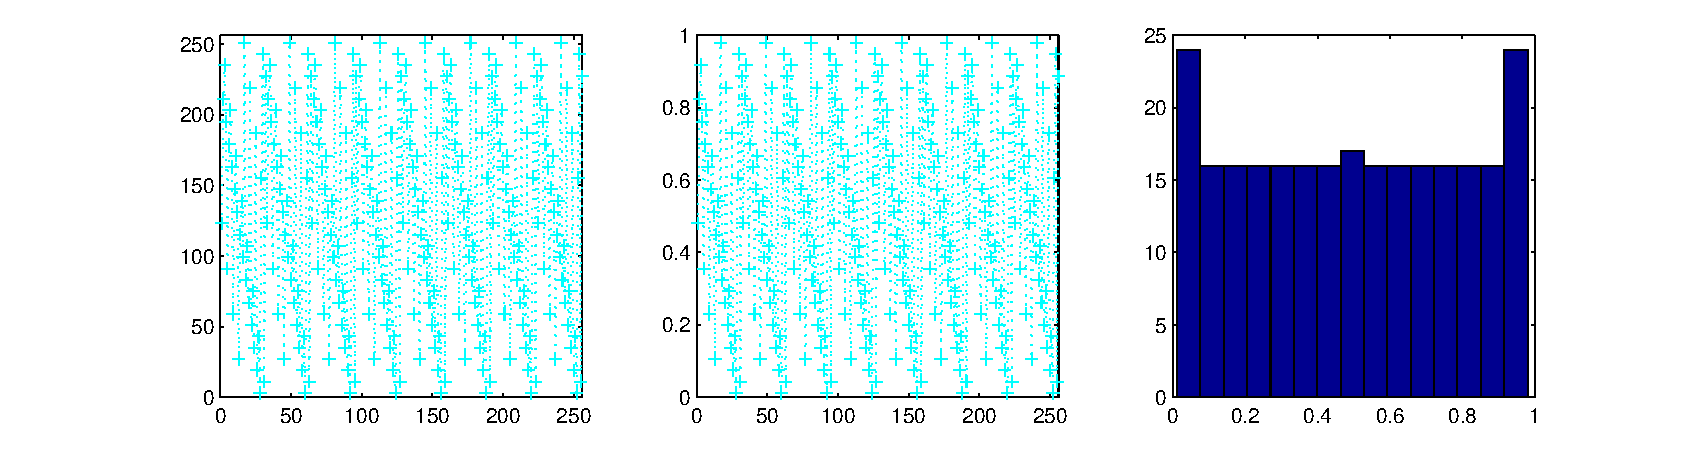
\includegraphics[width=7.0in]{figures/LinConGenKnuth334T1L5Plots}}
\end{figure}


\subsubsection*{Choosing the {\em suitable} magic input $(m,a,c,x_0,n)$}

The linear congruential  generator is a special case of a {\em discrete dynamical system}: 
\[
x_{i}  = f(x_{i-1}), \ f: \{0,1,2,\ldots,m-1\} \to \{0,1,2,\ldots,m-1\} \ \text{and} \ f(x_{i-1})=(a x_{i-1} + c) \mod m\enspace .
\]  
Since $f$ maps a the finite set $\{1,2,\ldots,m-1\}$ into itself, such systems are bound to have a repeating cycle of numbers called the {\bf period}.  In Labwork~\ref{LW:GenericLCGS}, the generator {\tt LinConGen(13,12,11,10,12)} has period $(10,1)$ of length $2$, the generator {\tt LinConGen (13,10,9,8,12)} has period $(8, 11, 2, 3, 0, 9)$ of length $6$ and the generator {\tt LinConGen(256,137,0,123,257)} has a period of length $32$.  All these generators have a non-maximal period length less than their modulus $m$.  A good generator should have a maximal period of $m$.  Let us try to implement a generator with a maximal period of $m=256$.


The period of a general LCG is at most $m$, and for some choices of $a$ the period can be much less than $m$ as shown in the examples considered earlier.  The LCG will have a full period if and only if:
\begin{enumerate}
\item $c$ and $m$  are relatively prime,
\item  $a-1$ is divisible by all prime factors of $m$,
\item  $a-1$ is a multiple of $4$ if  $m$ is a multiple of $4$
\end{enumerate}

\begin{labwork}[LCG with maximal period length of $256$]
Consider the linear congruential sequence with $(m,a,c,x_0,n)= (256,137,123,13,256)$.  First check that these parameters do indeed satisfy the three condition above and therefore can produce the maximal period length of only $m=256$.  Modify the input parameter to {\tt LinConGen} and repeat Labwork~\ref{LW:LinConGenKnuth334T1L5} in order to first produce a sequence of length $257$.  Do you see that the period is of maximal length of $256$ as opposed to the generator of Labwork~\ref{LW:LinConGenKnuth334T1L5}?  Next produce a Figure to visualise the sequence as done in Figure~\ref{F:LinConGenKnuth334T1L5Plots}.
\end{labwork}

A useful sequence should clearly have a relatively long period, say at least $2^{30}$.  Therefore, the {\bf modulus $m$ has to be rather large} because the {\bf period} cannot have more than $m$ elements.  Moreover, the quality of pseudo-random numbers of a LCG is extremely sensitive to the choice of $m$, $a$ and $c$ even if the maximal period is attained.  The next example illustrates this point.

\begin{labwork}[The infamous {\tt RANDU}]\label{LW:RANDU}
{\tt RANDU} is an infamous LCG, which has been used since the 1960s.  It is widely considered to be one of the most ill-conceived random number generators designed. Notably, it fails the {\bf spectral test} badly for dimensions greater than 2.  The following commands help visualise the sequence of first $5001/3$ triplets $(x_i,x_{i+1},x_{i+2})$ seeded from $x_0=1$ (Figure~\ref{F:RANDU3D5001pts}).  Read {\tt help reshape} and {\tt help plot3}. 
\begin{VrbM}
>> x=reshape( (LinConGen(2147483648,65539,0,1,5001)./ 2147483648) ,3,[]);
>> plot3(x(1,:),x(2,:),x(3,:),'.')
\end{VrbM}
\end{labwork}

\begin{figure}[htbp]
\caption{The LCG called {\tt RANDU} with $(m,a,c)=(2147483648,65539,0)$ has strong correlation between three consecutive points as: $x_{i+2}=6x_{k+1}-9x_k$.  The two plots are showing $(x_i,x_{i+1},x_{i+2})$ from two different view points.
.\label{F:RANDU3D5001pts}}
\centering   \makebox{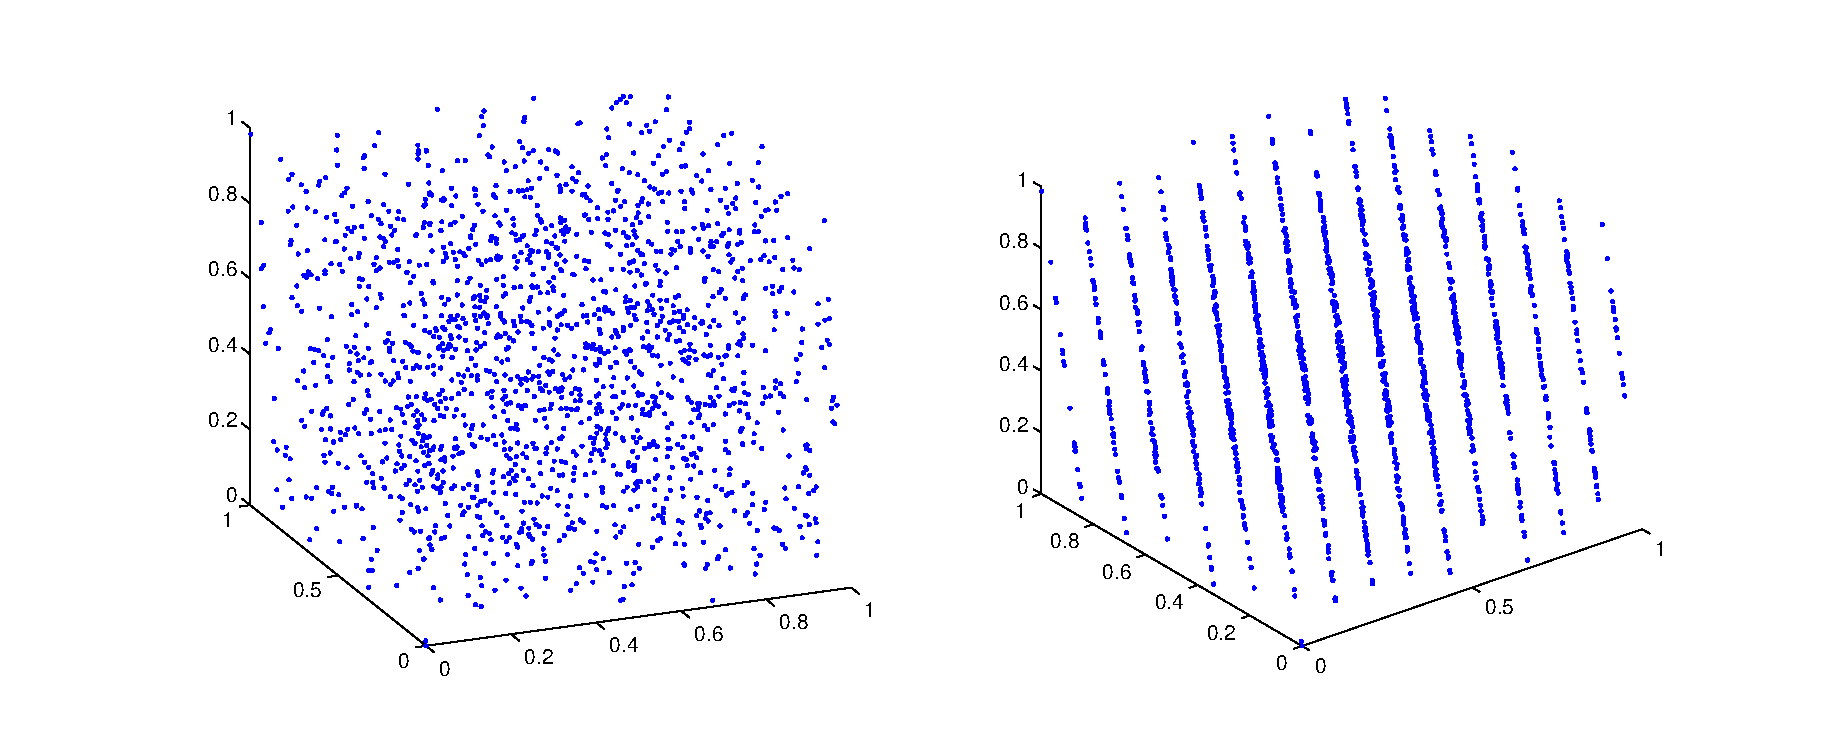
\includegraphics[width=7.0in]{figures/RANDU3D5001pts}}
\end{figure}

\begin{labwork}[Fishman20 and Lecuyer21 LCGs]
The following two LCGs are recommended in Knuth's Art of Computer Programming, vol.~2, for generating pseudo-random numbers for simple simulation tasks.
\begin{VrbM}
>> LinConGen(2147483647,48271,0,08787458,10) ./ 2147483647
ans =    0.0041    0.5239    0.0755    0.7624    0.6496    0.0769    0.9030    0.4259    0.9948    0.8868

>> LinConGen(2147483399,40692,0,01234567,10) ./ 2147483399
ans =    0.0006    0.3934    0.4117    0.7893    0.3913    0.6942    0.6790    0.3337    0.2192    0.1883
\end{VrbM}
\end{labwork}

The number of random numbers $n$ should at most be about $m/1000$ in order to avoid the future sequence from behaving like the past.  Thus, if $m=2^{32}$ then a new generator, with a new suitable set of $(m,a,c,x_0,n)$ should be adopted after the consumption of every few million pseudo-random numbers.

The LCGs are the least sophisticated type of PRNGs.  They are easier to understand but are not recommended for intensive simulation purposes.  The next section briefly introduces a more sophisticated PRNG we will be using in this course.  Moreover our implementation of LCGs using the variable precision integer package is extremely slow in {\sc MATLAB} and is only of pedagogical interest. 

\subsection{Generalized Feedback Shift Register  and the``Mersenne Twister'' PRNG} 

The following generator termed {\tt twister} in {\sc Matlab} is recommended for use in simulation.  It has extremely long periods, low correlation and passes most statistical tests (the {\sc diehard} statistical tests).  The {\tt twister} random number generator of Makoto Matsumoto and Takuji Nishimura is a variant of the twisted generalized feedback shift-register algorithm, and is known as the ``Mersenne Twister'' generator [Makoto Matsumoto and Takuji Nishimura, {\em Mersenne Twister: A 623-dimensionally equidistributed uniform pseudorandom number generator}, ACM Transactions on Modeling and Computer
Simulation, Vol.~8, No.~1 (Jan.~1998), Pages 3--30].  It has a Mersenne prime period of $2^{19937} - 1$ (about $10^{6000}$) and is {\bf equi-distributed} in $623$ dimensions.  It uses $624$ words of state per generator and is comparable in speed to the other generators.  The recommended default seed is $5489$.  See \url{http://www.math.sci.hiroshima-u.ac.jp/~m-mat/MT/emt.html} and \url{http://en.wikipedia.org/wiki/Mersenne_twister} for details.  

Let us learn to implement the {\sc Matlab} function that generates PRNs.  In {\sc Matlab} the function {\tt rand} produces a deterministic PRN sequence.  First, read {\tt help rand}.  We can generate PRNs as follows.
\begin{labwork}[Calling PRNG in {\sc Matlab}]\label{LW:RNGMatlab}
In {\sc Matlab} {\tt rand} is basic PRNG command.
\begin{VrbM}
>> rand(1,10) % generate a 1 X 10 array of PRNs
ans =
    0.8147    0.9058    0.1270    0.9134    0.6324    0.0975    0.2785    0.5469    0.9575    0.9649
>> rand(1,10) % generate another 1 X 10 array of PRNs
ans =
    0.1576    0.9706    0.9572    0.4854    0.8003    0.1419    0.4218    0.9157    0.7922    0.9595
>> rand('twister',5489) % reset the PRNG to default state Mersenne Twister with seed=5489
>> rand(1,10) % reproduce the first array
ans =
    0.8147    0.9058    0.1270    0.9134    0.6324    0.0975    0.2785    0.5469    0.9575    0.9649
>> rand(1,10) % reproduce the second array
ans =
    0.1576    0.9706    0.9572    0.4854    0.8003    0.1419    0.4218    0.9157    0.7922    0.9595
\end{VrbM}  
In general, you can use any seed value to initiate your PRNG.  You may use the {\tt clock} command to set the seed:
\begin{VrbM}
>> SeedFromClock=sum(100*clock); % save the seed from clock
>> rand('twister',SeedFromClock) % initialize the PRNG
>> rand(1,10)
ans =
    0.3696    0.3974    0.6428    0.6651    0.6961    0.7311    0.8982    0.6656    0.6991    0.8606
>> rand(2,10)
ans =
    0.3432    0.9511    0.3477    0.1007    0.8880    0.0853    0.6067    0.6976    0.4756    0.1523
    0.5827    0.5685    0.0125    0.1555    0.5551    0.8994    0.2502    0.5955    0.5960    0.5700
>> rand('twister',SeedFromClock) % initialize the PRNG to same SeedFromClock
>> rand(1,10)
ans =
    0.3696    0.3974    0.6428    0.6651    0.6961    0.7311    0.8982    0.6656    0.6991    0.8606
\end{VrbM}
\end{labwork}
 
\begin{figure}[htbp]
\caption{Triplet point clouds from the ``Mersenne Twister'' with two different seeds (see Labwork~\ref{LW:3DPlotsMersenneTwister}).
.\label{F:MersenneTwisterTwo3DPtclouds}}
\centering   \makebox{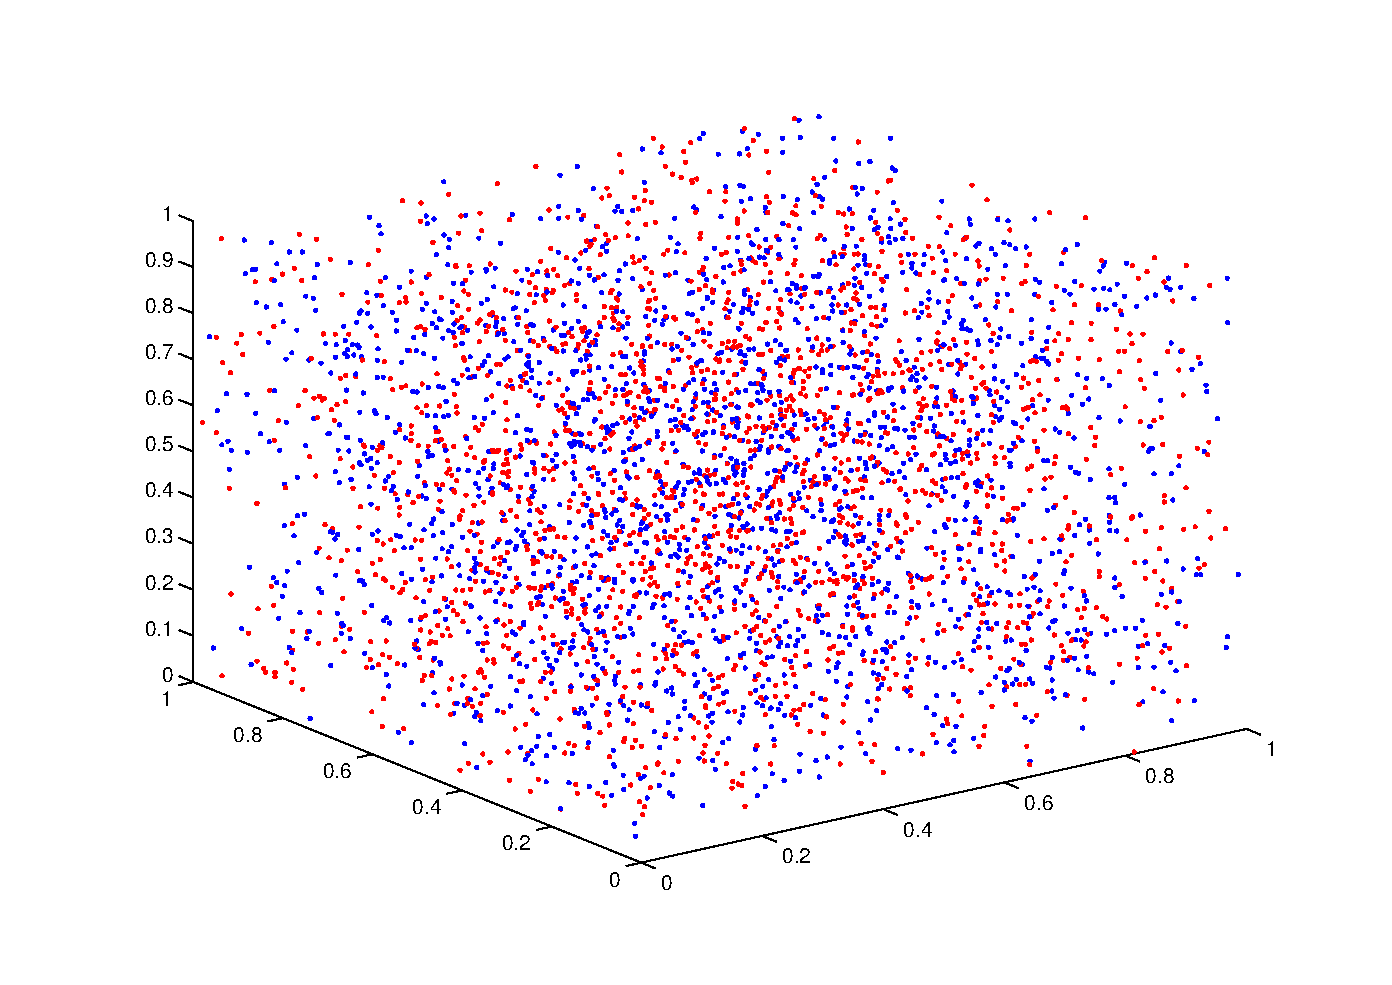
\includegraphics[width=6.0in]{figures/MersenneTwisterTwo3DPtclouds}}
\end{figure}
\begin{labwork}[3D plots of triplets generated by the ``Mersenne Twister'']\label{LW:3DPlotsMersenneTwister}
Try to find any correlation between triplets generated by the ``Mersenne Twister'' by rotating the 3D plot generated by the following code:
\begin{VrbM}
>> rand('twister',1234)
>> x=rand(3,2000); % store PRNs in a 3X2000 matrix named x
>> plot3(x(1,:),x(2,:),x(3,:),'.')
\end{VrbM}
Compare this with the 3D plot of triplets from {\tt RANDU} of Labwork~\ref{LW:RANDU}. Which of these two PRNGs do you think is ``more random'' looking? and why? 

Change the seed value to the recommended default by the authors and look at the point cloud (in red) relative to the previous point cloud (in blue).  Rotate the plots to visualise from multiple angles.  Are they still random looking?
\begin{VrbM}
>> rand('twister',1234)% same seed as before
>> x=rand(3,2000); % store PRNs in a 3X2000 matrix named x
>> rand('twister',5489)% the recommended default seed
>> y=rand(3,2000);% store PRNs seeded by 5489 in a 3X2000 matrix named y
>> plot3(x(1,:),x(2,:),x(3,:),'b.') % plot triplets as blue dots
>> hold on;
>> plot3(y(1,:),y(2,:),y(3,:),'r.') % plot triplets as red dots
\end{VrbM}
\end{labwork}

\section{Simulation of non-$\uniform(0,1)$ Random Variables}\label{S:nonUniformRVG}

%\remove{
The $\uniform(0,1)$ RV of \hyperref[M:Uniform01]{Model \ref*{M:Uniform01}} forms the foundation for random variate generation and simulation.  This is appropriately called the fundamental model or experiment, since every other experiment can be obtained from this one.

Next, we simulate or generate samples from other RVs by making the following two assumptions:
\begin{enumerate}
\item independent samples from the $\uniform(0,1)$ RV can be generated, and
\item real arithmetic can be performed exactly in a computer.
\end{enumerate}
Both these assumptions are, in fact, not true and require a more careful treatment of the subject.  We may return to these careful treatments later on.

\subsection{Inversion Sampler for Continuous Random Variables}\label{S:InvS}
\begin{prop}[Inversion sampler]\label{P:InvS}
Let $F(x) := \int_{- \infty}^{x} f(y) \,d y : \Rz \rightarrow [0,1]$ be a continuous DF with density $f$, and let its inverse $F^{[-1]} : [0,1] \rightarrow \Rz $ be:
\[
F^{[-1]}(u) :=  \inf \{ x :  F(x) = u \} \ .
\]
Then, $F^{[-1]}(U)$ has the distribution function $F$, provided $U$ is a $\uniform(0,1)$ RV.  Recall $\inf(A)$ or infimum of a set $A$ of real numbers is the greatest lower bound of every element of $A$.
\end{prop}
\begin{proof}
The ``one-line proof'' of the proposition is due to the following equalities:
\[
\p(F^{[-1]}(U) \leq x) = \p(\inf \{ y :  F(y) = U)\} \leq x ) = \p(U \leq F(x)) = F(x), \quad for~all~x \in \Rz .
\]
\end{proof}

This yields the inversion sampler or the inverse (C)DF sampler, where we (i) {\it generate} $u \sim \uniform(0,1)$ and (ii) {\it return} $x = F^{[-1]}(u)$, as formalised by the following algorithm.

\begin{algorithm}
\caption{Inversion Sampler or Inverse (C)DF Sampler}
\label{A:InvS}
\begin{algorithmic}[1]
\STATE {
{\it input:}
(1) $F^{[-1]}(x)$, inverse of the DF of the target RV $X$,
(2) the fundamental sampler
}
\STATE {\it initialise:} set the seed, if any, for the fundamental sampler
\STATE {\it output:} a sample from $X$ distributed according to $F$
\STATE {{\it draw} $u \sim \uniform(0,1)$}
\STATE {\it return:} $x = F^{[-1]}(u)$
\end{algorithmic}
\end{algorithm}
This algorithm emphasises the fundamental sampler's availability in an {\it input} step, and its set-up needs in an {\it initialise} step.  In the following sections, we will not mention these universal steps; they will be taken for granted.  The direct applicability of \hyperref[A:InvS]{Algorithm \ref*{A:InvS}} is limited to univariate densities for which the inverse of the cumulative distribution function is explicitly known.  The next section will consider some examples.

%\section{Some Simulations of Continuous Random Variables}\label{S:InvSContinuousRVs}
%}%end remove
%\section{Continuous Random Variables}

Recall the $\uniform(\theta_1,\theta_2)$ RV of \hyperref[M:Uniformab]{Model \ref*{M:Uniformab}} with the following PDF, DFand inverse DF. Let us simulate from it using the inversion sampler.

\begin{figure}[htpb]
\caption{A plot of the PDF, DF or CDF and inverse DF of the $\uniform(-1,1)$ RV $X$.\label{F:unifpm1}}
\centering   \makebox{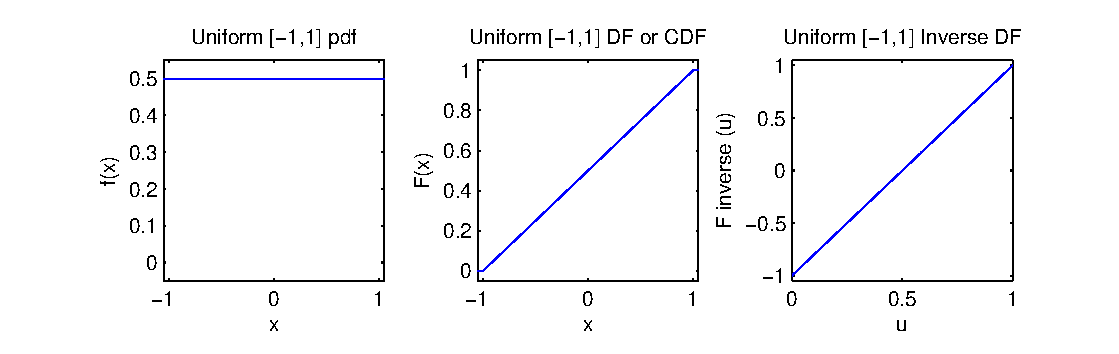
\includegraphics[width=6.5in]{figures/Unifpm1pdfcdf}}
\end{figure}

\begin{simulation}[$\uniform(\theta_1,\theta_2)$]\label{SIM:Uniformab}
To simulate from $\uniform(\theta_1,\theta_2)$ RV $X$ using the Inversion Sampler, we first need to find $F^{[-1]}(u)$ by solving for $x$ in terms of $u=F(x;\theta_1,\theta_2)$:
\[
u = \frac{x-\theta_1}{\theta_2-\theta_1} \quad \iff  \quad x = (\theta_2-\theta_1)u+\theta_1 \quad  \iff \quad  F^{[-1]}(u;\theta_1,\theta_2) = \theta_1+(\theta_2-\theta_1)u
\]
Here is a simple implementation of the Inversion Sampler for the $\uniform(\theta_1,\theta_2)$ RV in \Matlab:
\begin{VrbM}
>> rand('twister',786); % initialise the fundamental sampler for Uniform(0,1)
>> theta1=-1; theta2=1; % declare values for parameters theta1 and theta2
>> u=rand; % rand is the Fundamental Sampler and u is a sample from it
>> x=theta1+(theta2 - theta1)*u; % sample from Uniform(-1,1]) RV
>> disp(x); % display the sample from Uniform[-1,,1] RV
    0.5134
\end{VrbM}
It is just as easy to draw $n$ IID samples from $\uniform(\theta_1,\theta_2)$ RV $X$ by transforming $n$ IID samples from the $\uniform(0,1)$ RV as follows:
\begin{VrbM}
>> rand('twister',786543); % initialise the fundamental sampler
>> theta1=-83; theta2=1004; % declare values for parameters a and b
>> u=rand(1,5); % now u is an array of 5 samples from Uniform(0,1)
>> x=theta1+(theta2 - theta1)*u; % x is an array of 5 samples from Uniform(-83,1004]) RV
>> disp(x); % display the 5 samples just drawn from Uniform(-83,1004) RV
  465.3065  111.4994   14.3535  724.8881  254.0168
\end{VrbM}
%Next, we write a \Matlab function for this sampler which would take the appropriate inputs and return $n$ IID samples from a specified $Uniform(\theta_1,\theta_2)$ RV $X$.
%\VrbMf[label=UniformabSam.m]{UniformabSam.m}
\end{simulation}

%\remove{
\begin{labwork}[Inversion Sampler Demo -- $\uniform(-5,5)$]\label{LW:guiInversionSamplerUniform}
Let us comprehend the inversion sampler by calling the interactive visual cognitive tool built by Jennifer Harlow under a grant from University of Canterbury's Centre for Teaching and Learning (UCTL):
\begin{VrbM}
>> guiInversionSampler
\end{VrbM}
The M-file {\tt guiInversionSampler.m} will bring a graphical user interface (GUI) as shown in \hyperref[F:guiInversionSamplerUniform]{Figure \ref*{F:guiInversionSamplerUniform}}.  The default target distribution is $\uniform(-5,5)$.  Now repeatedly push the ``Draw one sample'' button several times and comprehend the simulation process.  You can press ``Draw 100 samples'' to really comprehend the inversion sampler in action after 100 samples are drawn and depicted in the density histogram of the accumulating samples.  
Next try changing the numbers in the ``Lower bound'' and ``Upper bound'' boxes in order to alter the parameters $\theta_1$ and $\theta_2$ of $\uniform(\theta_1,\theta_2)$ RV.  
\end{labwork}

\begin{figure}[htpb]
\caption{Visual Cognitive Tool GUI: Inversion Sampling from $X \sim \uniform(-5,5)$.\label{F:guiInversionSamplerUniform}}
\centering   \makebox{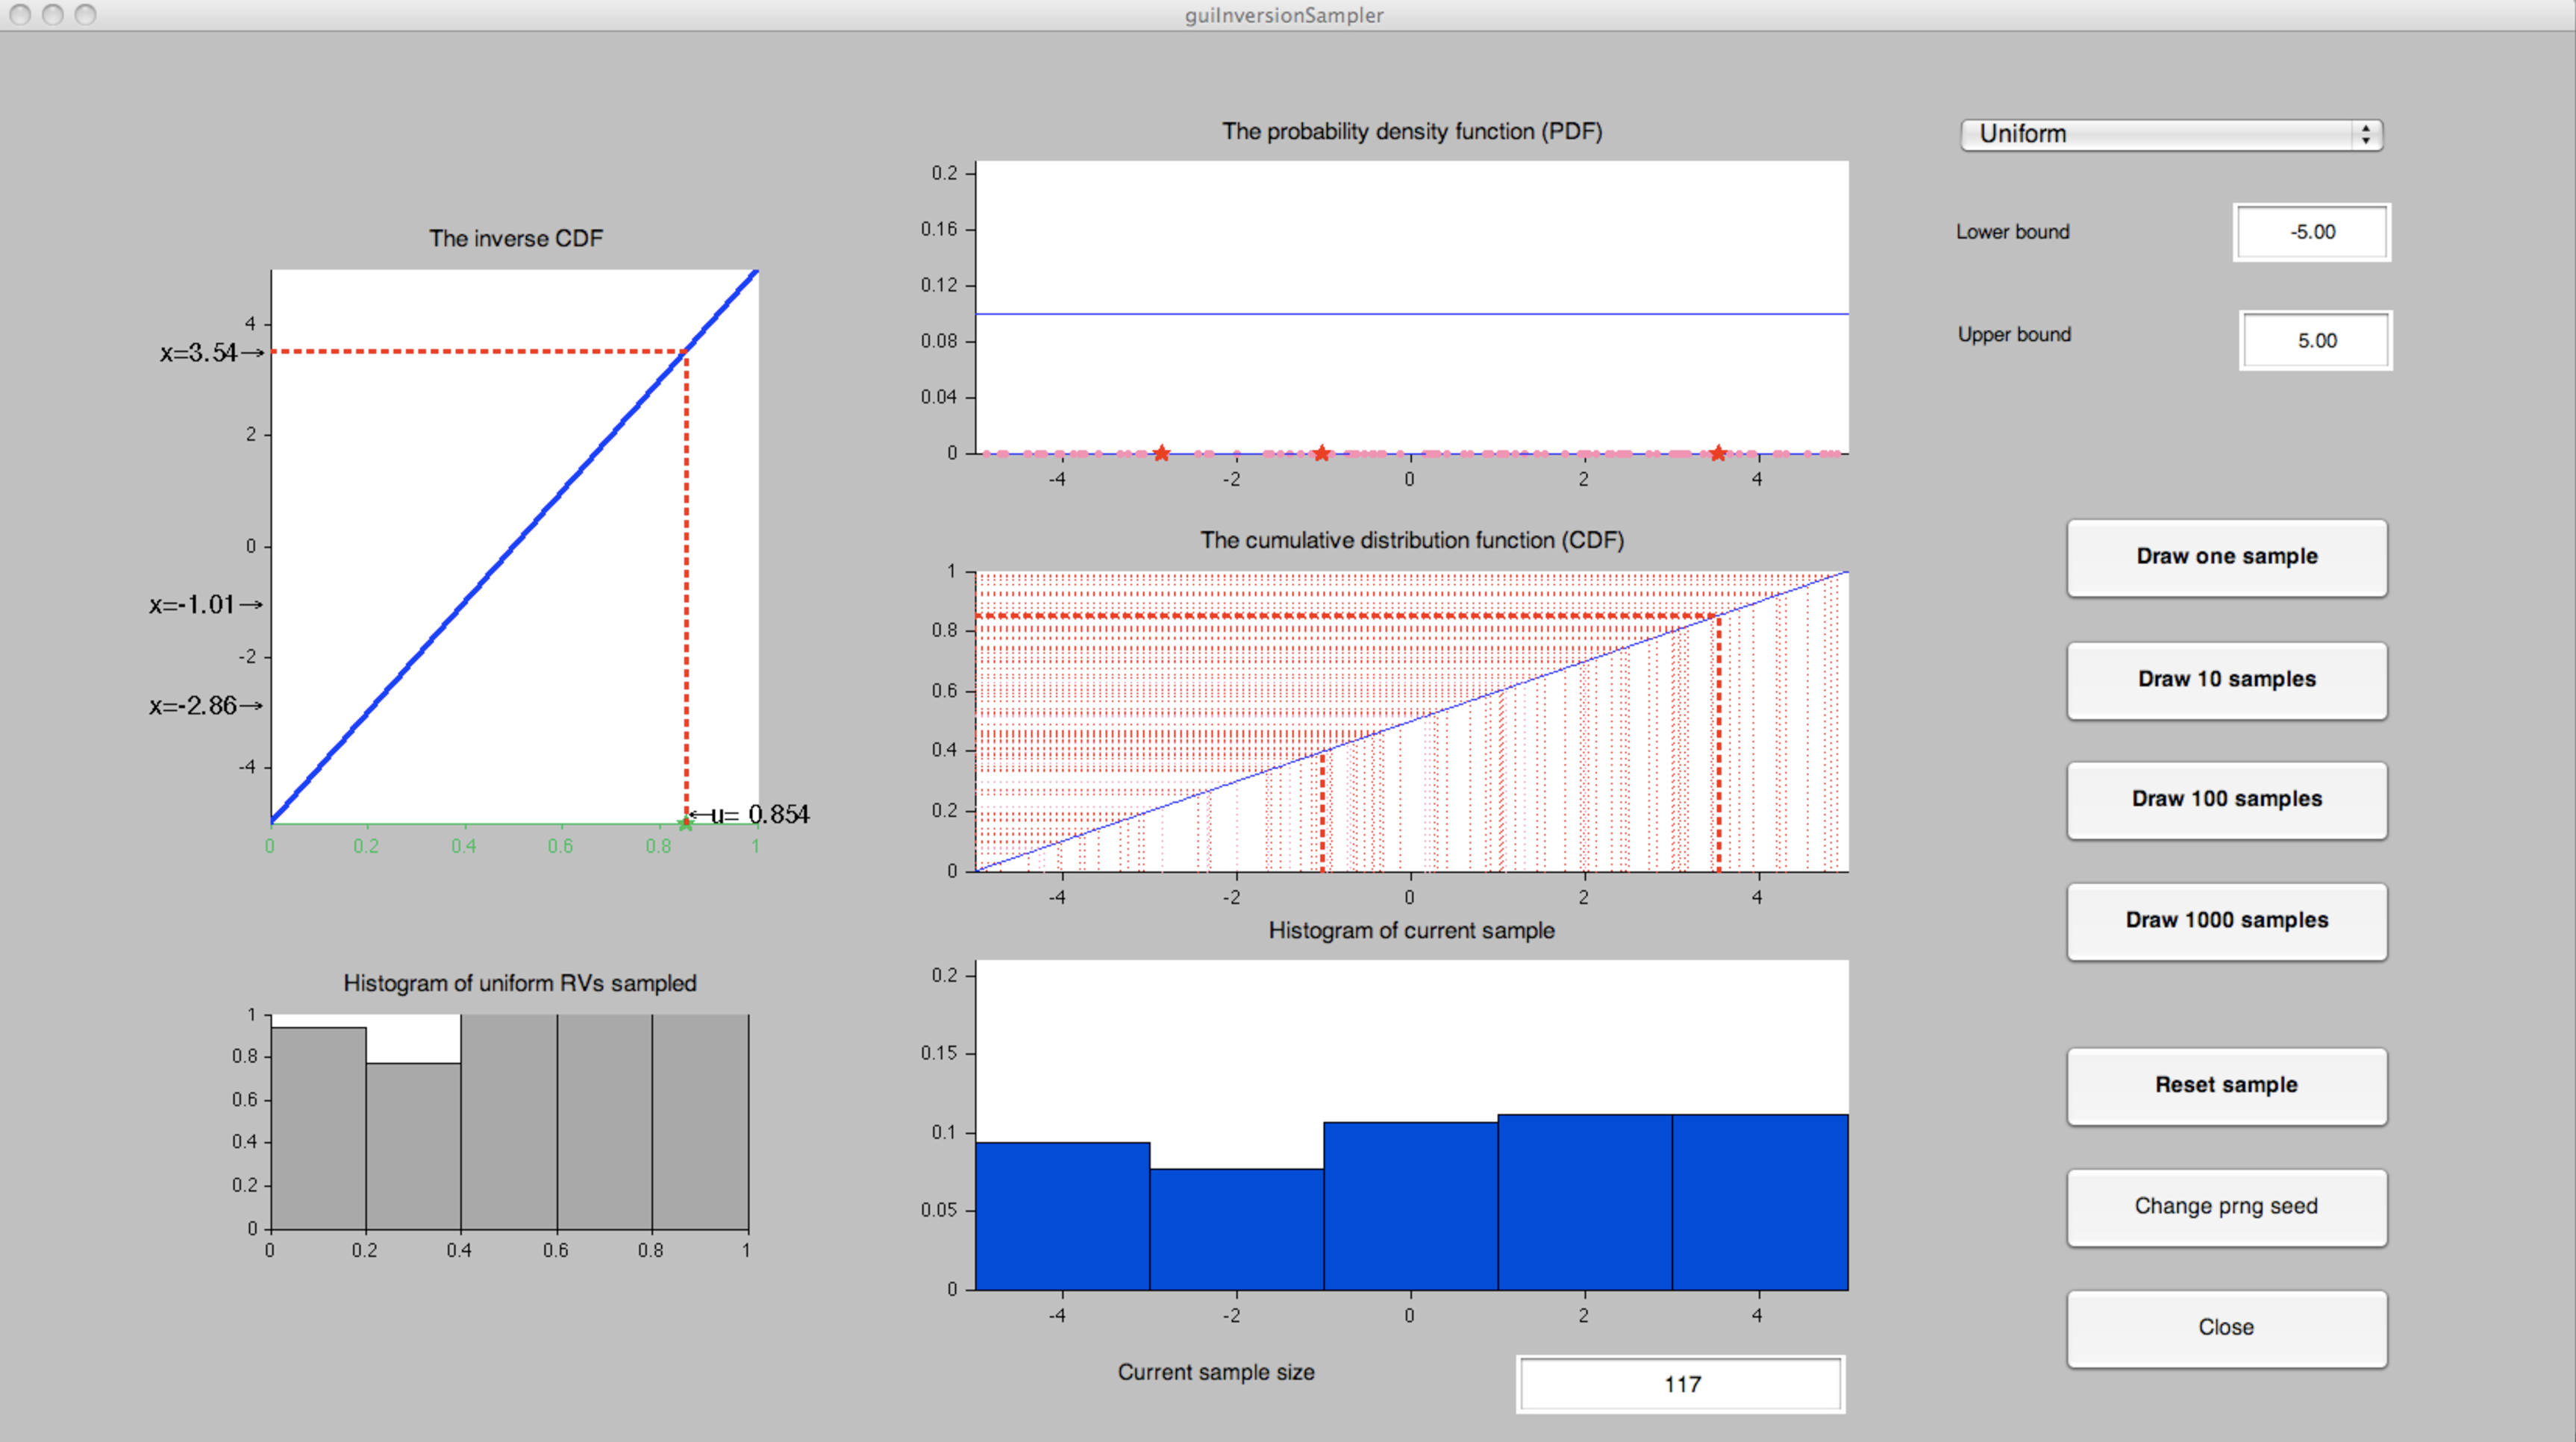
\includegraphics[width=6.50in]{figures/guiInversionSamplerUniform}}
\end{figure}

%}%end remove

Recall the $\exponential(\lambda)$ RV of \hyperref[M:exponential]{Model \ref*{M:exponential}}. Let us simulate from it using the inversion sampler.

\begin{figure}[htpb]
\caption{The PDF $f$, DF $F$, and inverse DF $F^{[-1]}$ of the the $\exponential(\lambda=1.0)$ RV. \label{F:ExpfFFInv}}
\centering   \makebox{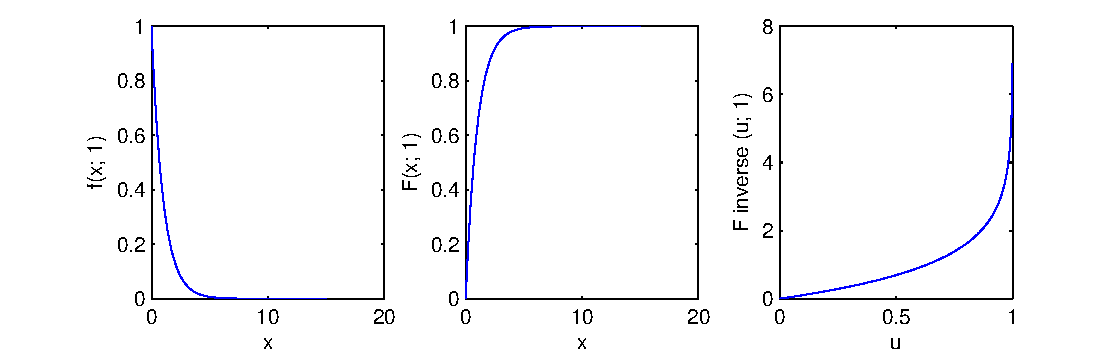
\includegraphics[width=6.5in]{figures/plotExpfFFInv}}
\end{figure}

Let us consider the problem of simulating from an $\exponential(\lambda)$ RV with realisations in $\Rz_+ := [0,\infty) := \{x: x \geq 0, x \in \Rz\}$ to model the waiting time for a bus at a bus stop.
\begin{simulation}[$\exponential(\lambda)$]\label{SIM:Exponential}
For a given $\lambda > 0$, an $\exponential(\lambda)$ RV has the following PDF $f$, DF $F$ and inverse DF $F^{[-1]}$:
\begin{eqnarray}
f(x; \lambda) = \lambda e^{-\lambda x} \quad &
F(x; \lambda)= 1-e^{-\lambda x} \quad &
F^{[-1]}(u; \lambda)= \frac{-1}{\lambda} \log_e (1-u)
\end{eqnarray}
We write the natural logarithm $\log_e$ as $\log$ for notational simplicity.  An implementation of the Inversion Sampler for $\exponential(\lambda)$ as a function in the M-file:
\VrbMf[label=ExpInvCDF.m]{scripts/ExpInvCDF.m}
We can simply call the function to draw a sample from, say the $\exponential(\lambda=1.0)$ RV by:
\begin{VrbM}
  lambda=1.0;			% some value for lambda
  u=rand;			% rand is the Fundamental Sampler
  ExpInvCDF(u,lambda)	% sample from Exponential(1) RV via function in ExpInvCDF.m
\end{VrbM}
Because of the following (recall \hyperref[Ex:1-UisU]{Example \ref*{Ex:1-UisU}}):
\[
 U \sim \uniform(0,1) \quad \implies \quad
 -U \sim \uniform(-1,0) \quad \implies \quad
 1-U \sim \uniform(0,1)  \  ,
 \]
 we could save a subtraction operation in the above algorithm by replacing {\tt -(1/lambda) * log(1-u)} by {\tt -(1/lambda) * log(u)}. 
Recall that the transformation of $U \sim \uniform(0,1)$ by $X=-(1/\lambda) \log(U)$ is exactly how we defined $X$ as the $\exponential(\lambda)$ RV in \hyperref[M:exponential]{Model \ref*{M:exponential}}. 
This is implemented as the following function.
 \VrbMf[label=ExpInvSam.m]{scripts/ExpInvSam.m}
\begin{VrbM}
>> rand('twister',46678); % initialise the fundamental sampler
>> Lambda=1.0;  % declare Lambda=1.0
>> x=ExpInvSam(rand(1,5),Lambda); % pass an array of 5 Uniform(0,1) samles from rand
>> disp(x); % display the Exponential(1.0) distributed samples
    0.5945    2.5956    0.9441    1.9015    1.3973
\end{VrbM}
 % Get a concrete understanding by implementing this simulation in Lab.
\end{simulation}

%\remove{
\begin{labwork}[Inversion Sampler Demo -- $\exponential(0.5)$]\label{LW:guiInversionSamplerExponential}
Let us understand the inversion sampler by calling the interactive visual cognitive tool:
\begin{VrbM}
>> guiInversionSampler
\end{VrbM}
The M-file {\tt guiInversionSampler.m} will bring a graphical user interface (GUI) as shown in \hyperref[F:guiInversionSamplerExponential]{Figure \ref*{F:guiInversionSamplerExponential}}.  First change the target distribution from the default $\uniform(-5,5)$ to $\exponential(0.5)$ from the drop-down menu.  Now push the ``Draw 10 samples'' button and comprehend the simulation process.  Next try changing the ``Rate Parameter'' from $0.5$ to $10.0$ for example  and generate several inversion samples and see the density histogram of the accumulating samples.  You can press ``Draw one sample'' to really comprehend the inversion sampler in action one step at a time.
\end{labwork}

\begin{figure}[htpb]
\caption{Visual Cognitive Tool GUI: Inversion Sampling from $X \sim \exponential(0.5)$.\label{F:guiInversionSamplerExponential}}
\centering   \makebox{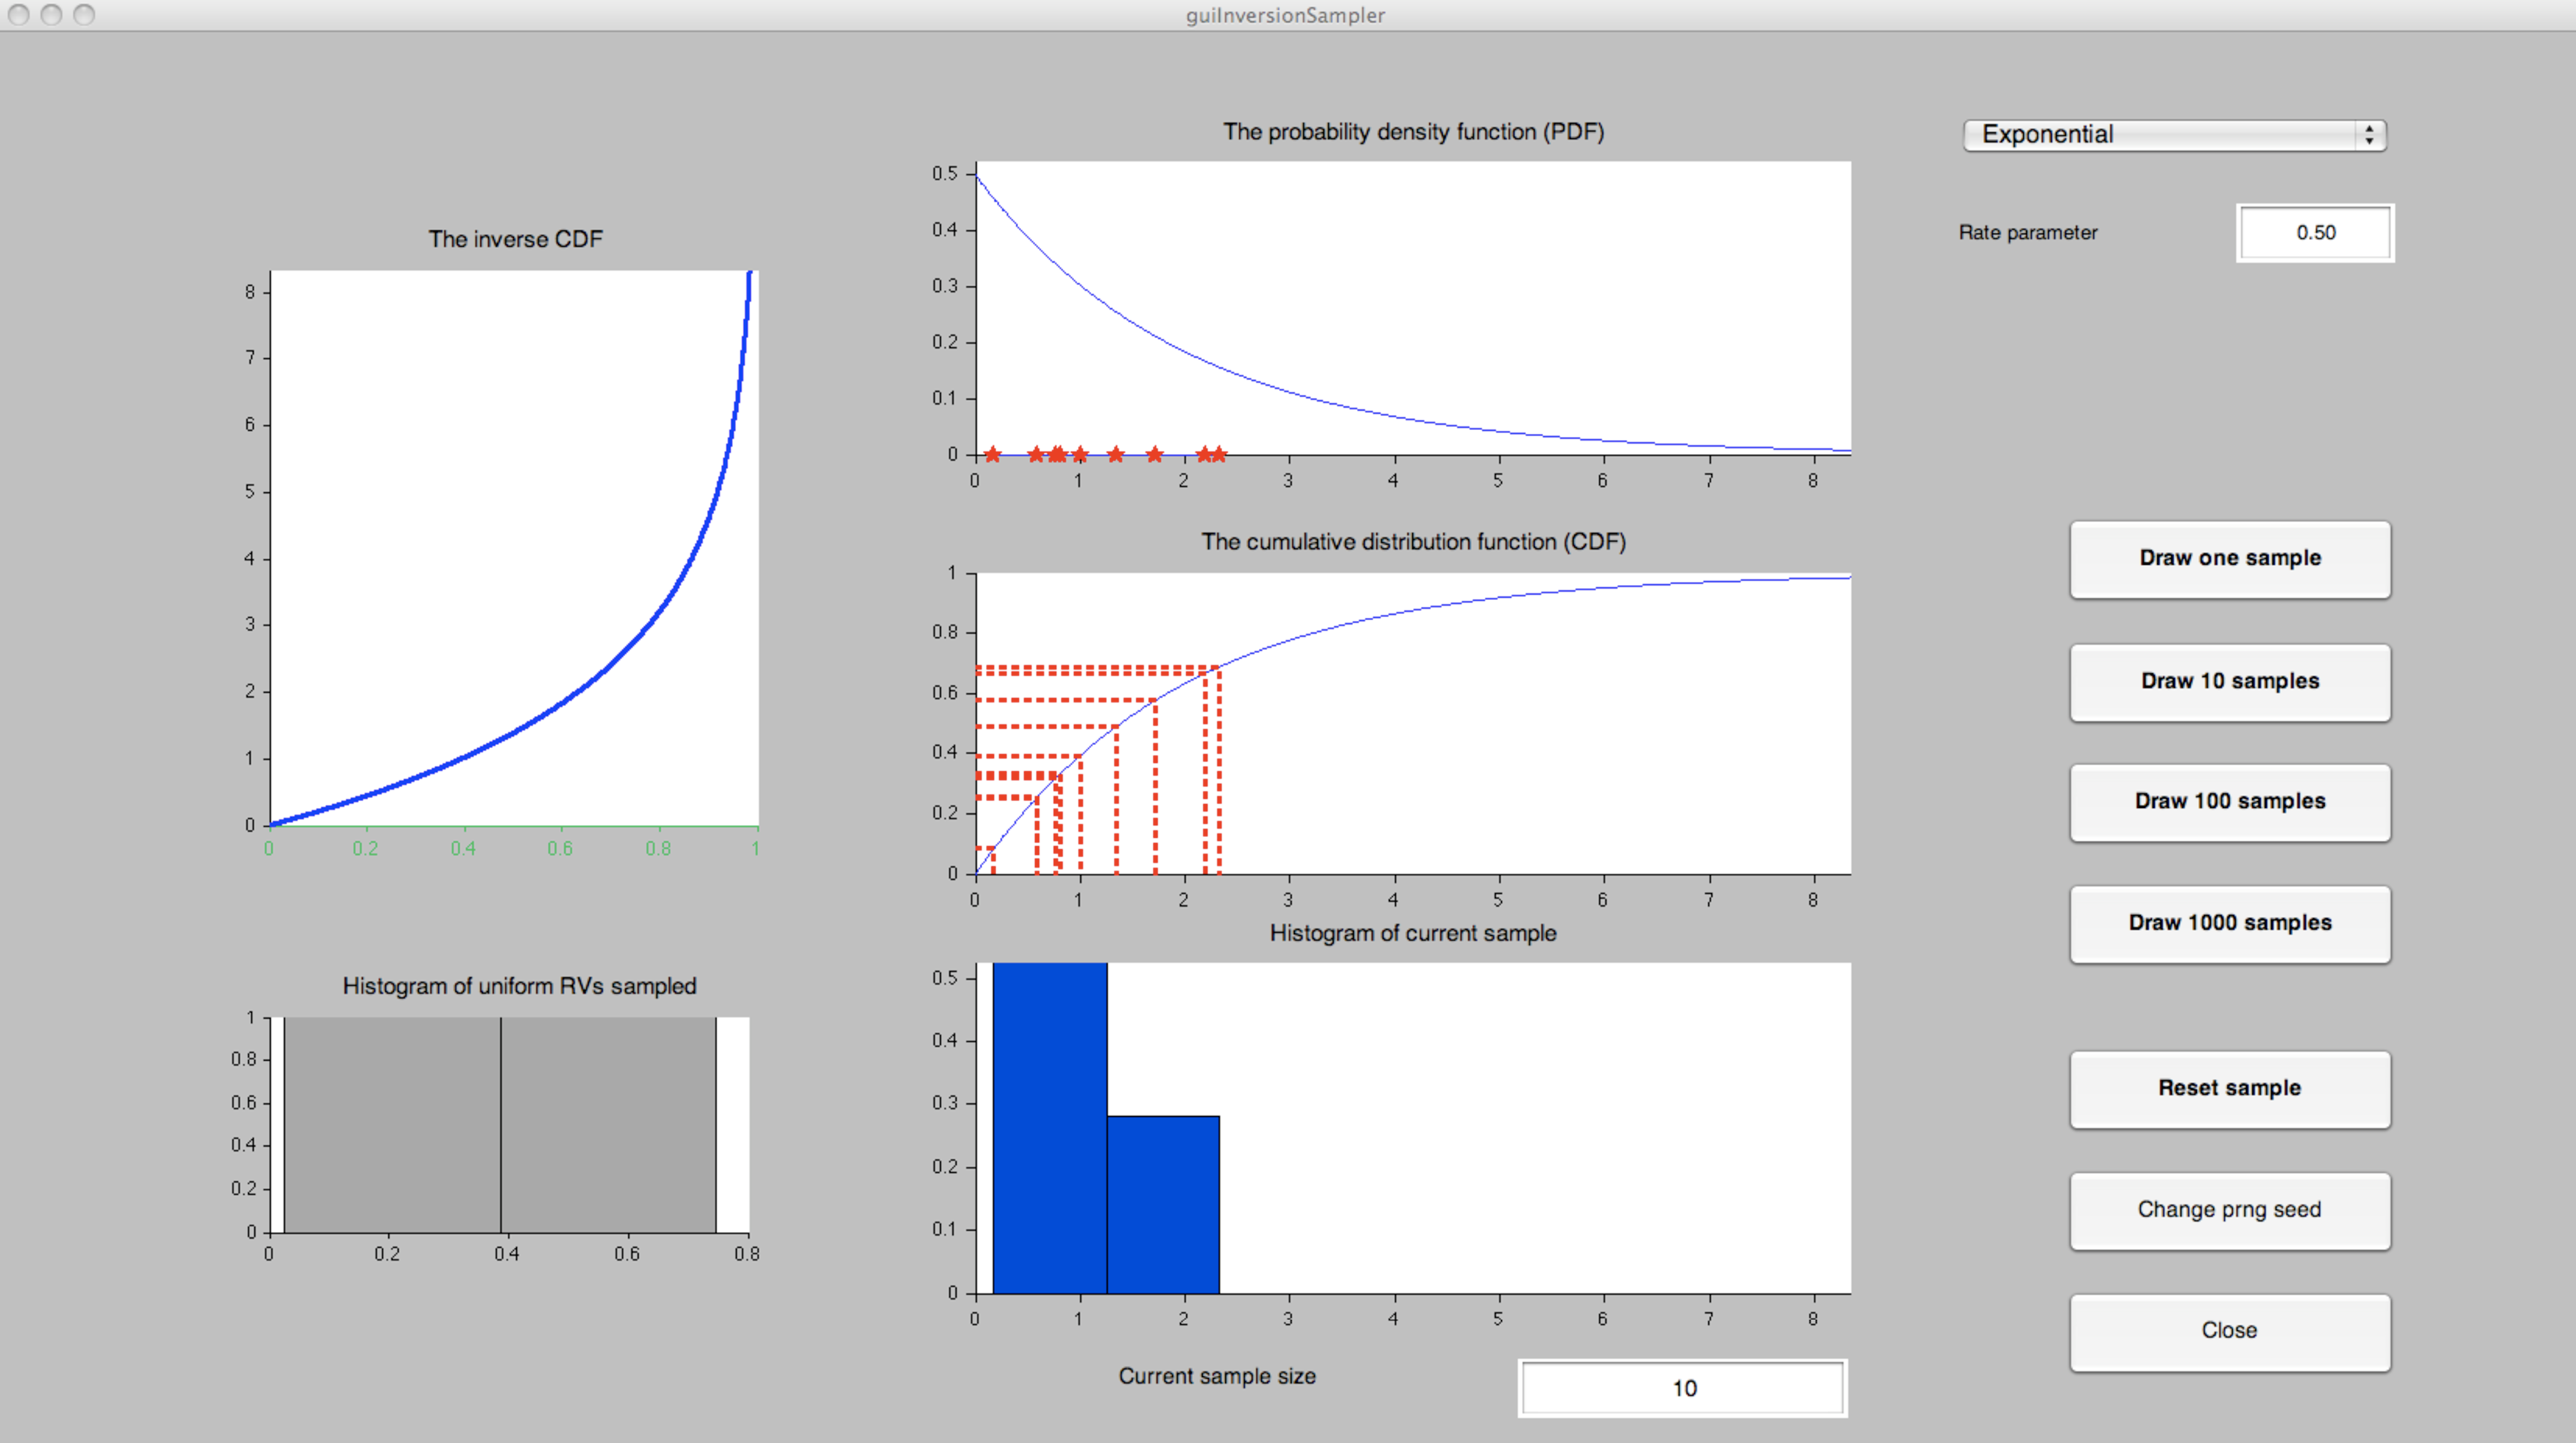
\includegraphics[width=6.50in]{figures/guiInversionSamplerExponential}}
\end{figure}
It is straightforward to do replicate experiments.  Consider the experiment of drawing five  independent samples from the $\exponential(\lambda=1.0)$ RV.  Suppose we want to repeat or replicate this experiment seven times and find the sum of the five outcomes in each of these replicates.  Then we may do the following:

\begin{VrbM}
>> rand('twister',1973); % initialise the fundamental sampler
>> % store 7 replications of 5 IID draws from Exponential(1.0) RV in array a
>> lambda=1.0; a= -1/lambda * log(rand(5,7)); disp(a);
    0.7267    0.3226    1.2649    0.4786    0.3774    0.0394    1.8210
    1.2698    0.4401    1.6745    1.4571    0.1786    0.4738    3.3690
    0.4204    0.1219    2.2182    3.6692    0.9654    0.0093    1.7126
    2.1427    0.1281    0.8500    1.4065    0.1160    0.1324    0.2635
    0.6620    1.1729    0.6301    0.6375    0.3793    0.6525    0.8330
>> %sum up the outcomes of the sequence of 5 draws in each replicate
>> s=sum(a); disp(s);
    5.2216    2.1856    6.6378    7.6490    2.0168    1.3073    7.9990
\end{VrbM}

\begin{labwork}[Next seven buses at your bus-stop]\label{LW:Next7Buses}
Consider the problem of modelling the arrival of buses at a bus stop.  Suppose that the time between arrivals is an $\exponential(\lambda=0.1)$ RV $X$ with a mean inter-arrival time of $1/\lambda=10$ minutes.  Suppose you go to your bus stop and zero a stop-watch.  Simulate the times of arrival for the next seven buses as indicated by your stop-watch.  Seed the fundamental sampler by your Student ID (eg.~if your ID is {\tt 11424620} then type {\tt rand('twister', 11424620);} just before the simulation).  Hand in the code with the arrival times of the next seven buses at your ID-seeded bus stop.
\end{labwork}

The support of the $\exponential(\lambda)$ RV is $\Rz_+ := [0,\infty)$.  Let us consider a RV built by mirroring the $\exponential(\lambda)$ RV about the origin with the entire real line as its support.
\begin{model}[$\laplace(\lambda)$ or $\doubleexponential(\lambda)$ RV]
If a RV $X$ is equally likely to be either positive or negative with an exponential density, then the $\laplace(\lambda)$ or $\doubleexponential(\lambda)$ RV, with the rate parameter $\lambda>0, \lambda \in \Rz$, may be used to model it.  The density function for the $\laplace(\lambda)$ RV given by $f(x; \lambda)$ is
\begin{equation}\label{E:Laplacepdf}
f(x; \lambda) = \frac{\lambda}{2} e^{- \lambda |x|} =
\begin{cases}
 \frac{\lambda}{2} e^{ \lambda x} & \text{if $x < 0$} \\
 \frac{\lambda}{2} e^{- \lambda x} & \text{if $x \geq 0$} \\
\end{cases}
\enspace .
\end{equation}
Let us define the sign of a real number $x$ by
\[
\sign(x) =
\begin{cases}
~~1 & \text{if $x > 0$} \\
~~0 & \text{if $x = 0$} \\
-1 & \text{if $x < 0$}  \ . \\
\end{cases}
\]
Then, the DF of the $\laplace(\lambda)$ RV $X$ is
\begin{equation} \label{E:Laplacecdf}
F(x; \lambda) = \int_{-\infty}^{x} f(y; \lambda)\,dy = \frac{1}{2}\left(1+ \sign(x) \left(1-e^{- \lambda |x|}\right) \right) \ ,
\end{equation}
and its inverse DF is
\begin{equation}\label{E:LaplaceInvcdf}
F^{[-1]}(u;\lambda) = - \frac{1}{\lambda} \ \sign\left(u-\frac{1}{2}\right) \log \left(1 - 2 \left|u-\frac{1}{2} \right| \right) \ , \ u \in [0,1]
\end{equation}
\end{model}

\paragraph{Mean and Variance of $\laplace(\lambda)$ RV $X$:}
Show that the mean of a $\laplace(\lambda)$ RV $X$ is
\[
\e(X) = \int_{0}^{\infty} x f(x;\lambda)\,dx
=   \int_{0}^{\infty} x \frac{\lambda}{2} e^{- \lambda |x|}\,dx
= 0 \ ,
\]
and the variance is
\[
\V(X) = \left(  \frac{1}{\lambda} \right)^2 + \left(  \frac{1}{\lambda} \right)^2 = 2 \left(  \frac{1}{\lambda} \right)^2\ .
\]
Note that the mean is $0$ due to the symmetry of the density about $0$ and the variance is twice that of the $\exponential(\lambda)$ RV.

\begin{labwork}[Rejection Sampler Demo -- $\laplace(5)$]\label{LW:guiInversionSamplerLaplace}
Let us comprehend the rejection sampler by calling the interactive visual cognitive tool:
\begin{VrbM}
>> guiInversionSampler
\end{VrbM}
The M-file {\tt guiInversionSampler.m} will bring a graphical user interface (GUI) as shown in \hyperref[F:guiInversionSamplerLaplace]{Figure \ref*{F:guiInversionSamplerLaplace}}.  Using the drop-down menu change from the default target distribution $\uniform(-5,5)$ to $\laplace(5)$.  Now repeatedly push the ``Draw one sample'' button several times and comprehend the simulation process.  You can also press ``Draw 1000 samples'' and see the density histogram of the generated samples.  
Next try changing the numbers in the ``Rate parameter'' box from $5.00$ to $1.00$ in order to alter the parameter $\lambda$ of $\laplace(\lambda)$ RV.  If you are more adventurous then try to alter the number in the ``Location parameter'' box from $0.00$ to some thing else, say $10.00$.  Although our formulation of $\laplace(\lambda)$ implicitly had a location parameter of $0.00$, we can easily introduce a location parameter $\mu$ into the PDF.  With a pencil and paper try to rewrite the PDF in \eqref{E:Laplacepdf} with an additional location parameter $\mu$.
\end{labwork}

\begin{figure}[htpb]
\caption{Visual Cognitive Tool GUI: Inversion Sampling from $X \sim \laplace(5)$.\label{F:guiInversionSamplerLaplace}}
\centering   \makebox{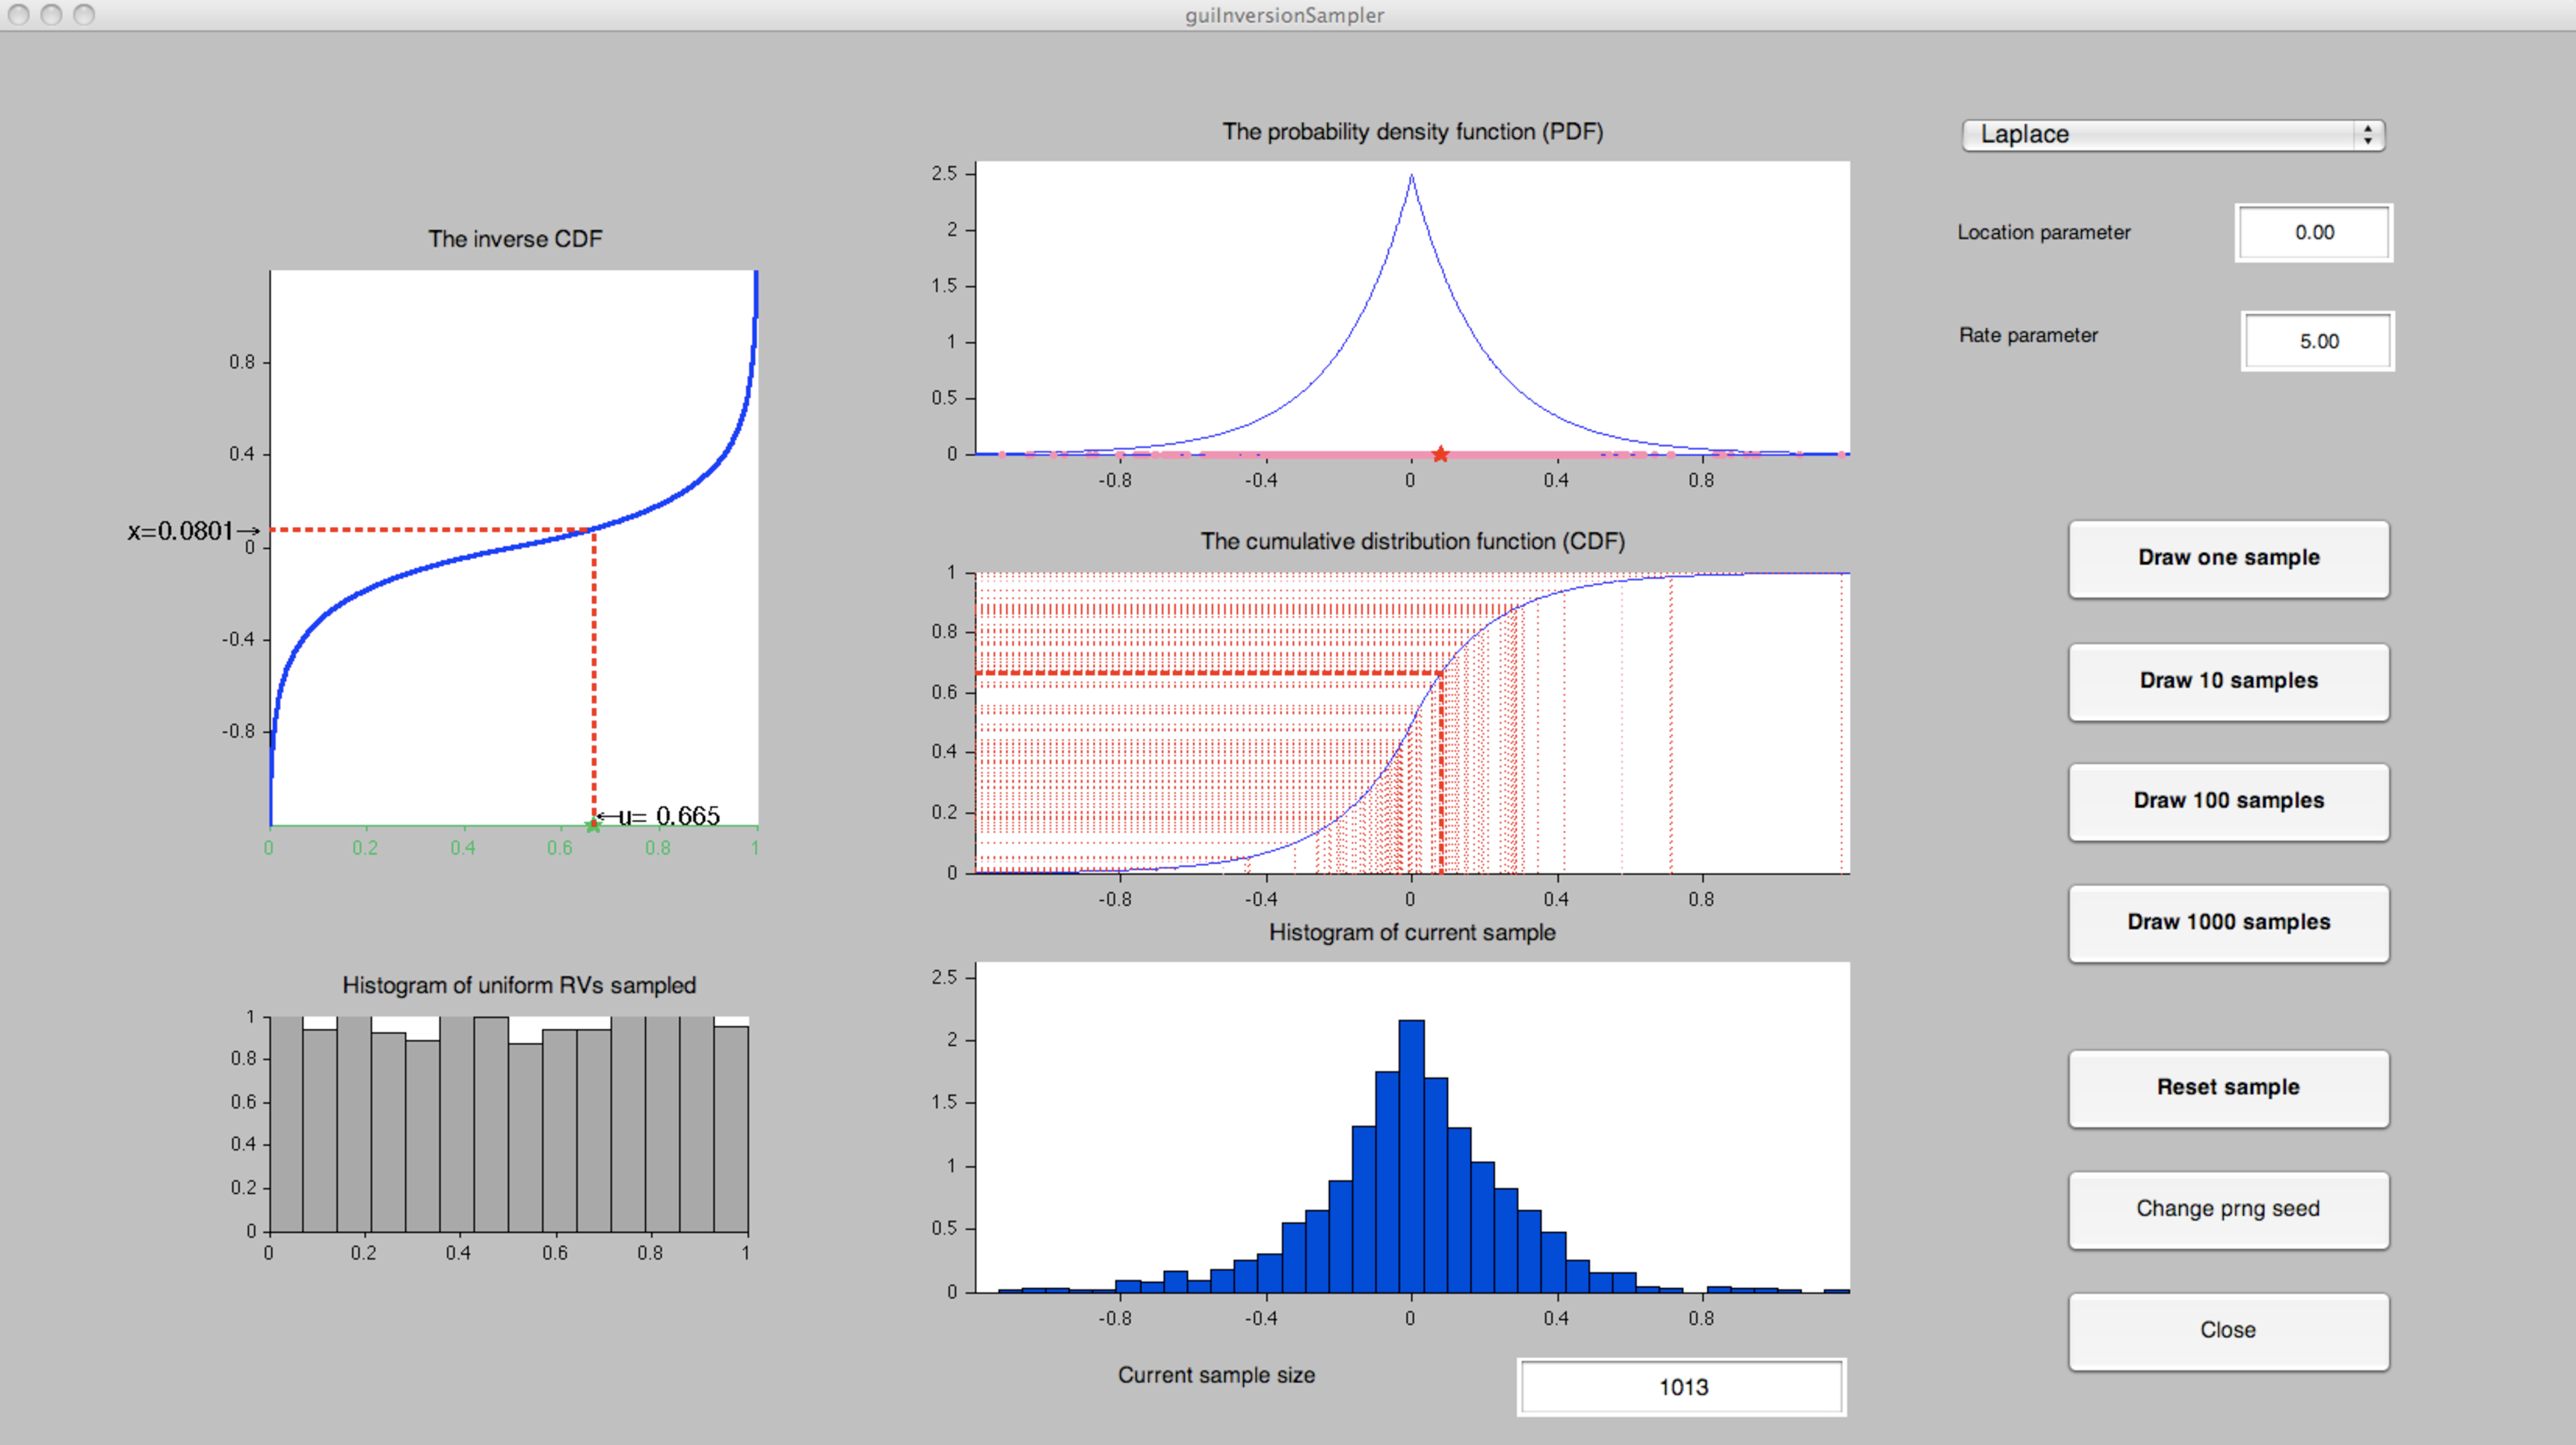
\includegraphics[width=6.50in]{figures/guiInversionSamplerLaplace}}
\end{figure}

\begin{simulation}[$\laplace(\lambda)$] \label{SIM:Laplace}
Here is an implementation of an inversion sampler to draw IID samples from a $\laplace(\lambda)$ RV $X$ by transforming IID samples from the $\uniform(0,1)$ RV $U$:
\VrbMf[label=LaplaceInvCDF.m]{scripts/LaplaceInvCDF.m}
We can simply call the function to draw a sample from, say the $\laplace(\lambda=1.0)$ RV by
\begin{VrbM}
>> lambda=1.0;		% some value for lambda
>> rand('twister',6567);        % initialize the fundamental sampler
>> u=rand(1,5);		% draw 5 IID samples from Uniform(0,1) RV
>> disp(u);		% display the samples in u
    0.6487    0.9003    0.3481    0.6524    0.8152

>> x=LaplaceInvCDF(u,lambda); % draw 5 samples from Laplace(1) RV using inverse CDF
>> disp(x);                     % display the samples
    0.3530    1.6127   -0.3621    0.3637    0.9953
\end{VrbM}
\end{simulation}

%}%end remove

%\remove{
\begin{labwork}[Inversion Sampler Demo -- $\cauchy$]\label{LW:guiInversionSamplerCauchy}
Let us comprehend the inversion sampler by calling the interactive visual cognitive tool:
\begin{VrbM}
>> guiInversionSampler
\end{VrbM}
The M-file {\tt guiInversionSampler.m} will bring a graphical user interface (GUI) as shown in \hyperref[F:guiInversionSamplerCauchy]{Figure \ref*{F:guiInversionSamplerCauchy}}.  Using the drop-down menu change from the default target distribution $\uniform(-5,5)$ to $\cauchy$ RV of Model~\ref{M:Cauchy}.  Now repeatedly push the ``Draw one sample'' button several times and comprehend the simulation process.  You can also press ``Draw 10 samples'' several times and see the density histogram of the generated samples.  
Next try changing the numbers in the ``Scale parameter'' and ``Location Parameter'' boxes from the default values of $1.00$ and  $0.00$, respectively.  Although our formulation of $\cauchy$ RV is also called {\em Standard Cauchy} as it implicitly had a location parameter of $0.00$ and scale parameter of $1$.  With a pencil and paper (in conjunction with a wikipedia search if you have to) try to rewrite the PDF in \eqref{E:StandardCauchypdf} with an additional location parameter $\mu$ and scale parameter $\sigma$.
\end{labwork}

\begin{figure}[htpb]
\caption{Visual Cognitive Tool GUI: Inversion Sampling from $X \sim \cauchy$.\label{F:guiInversionSamplerCauchy}}
\centering   \makebox{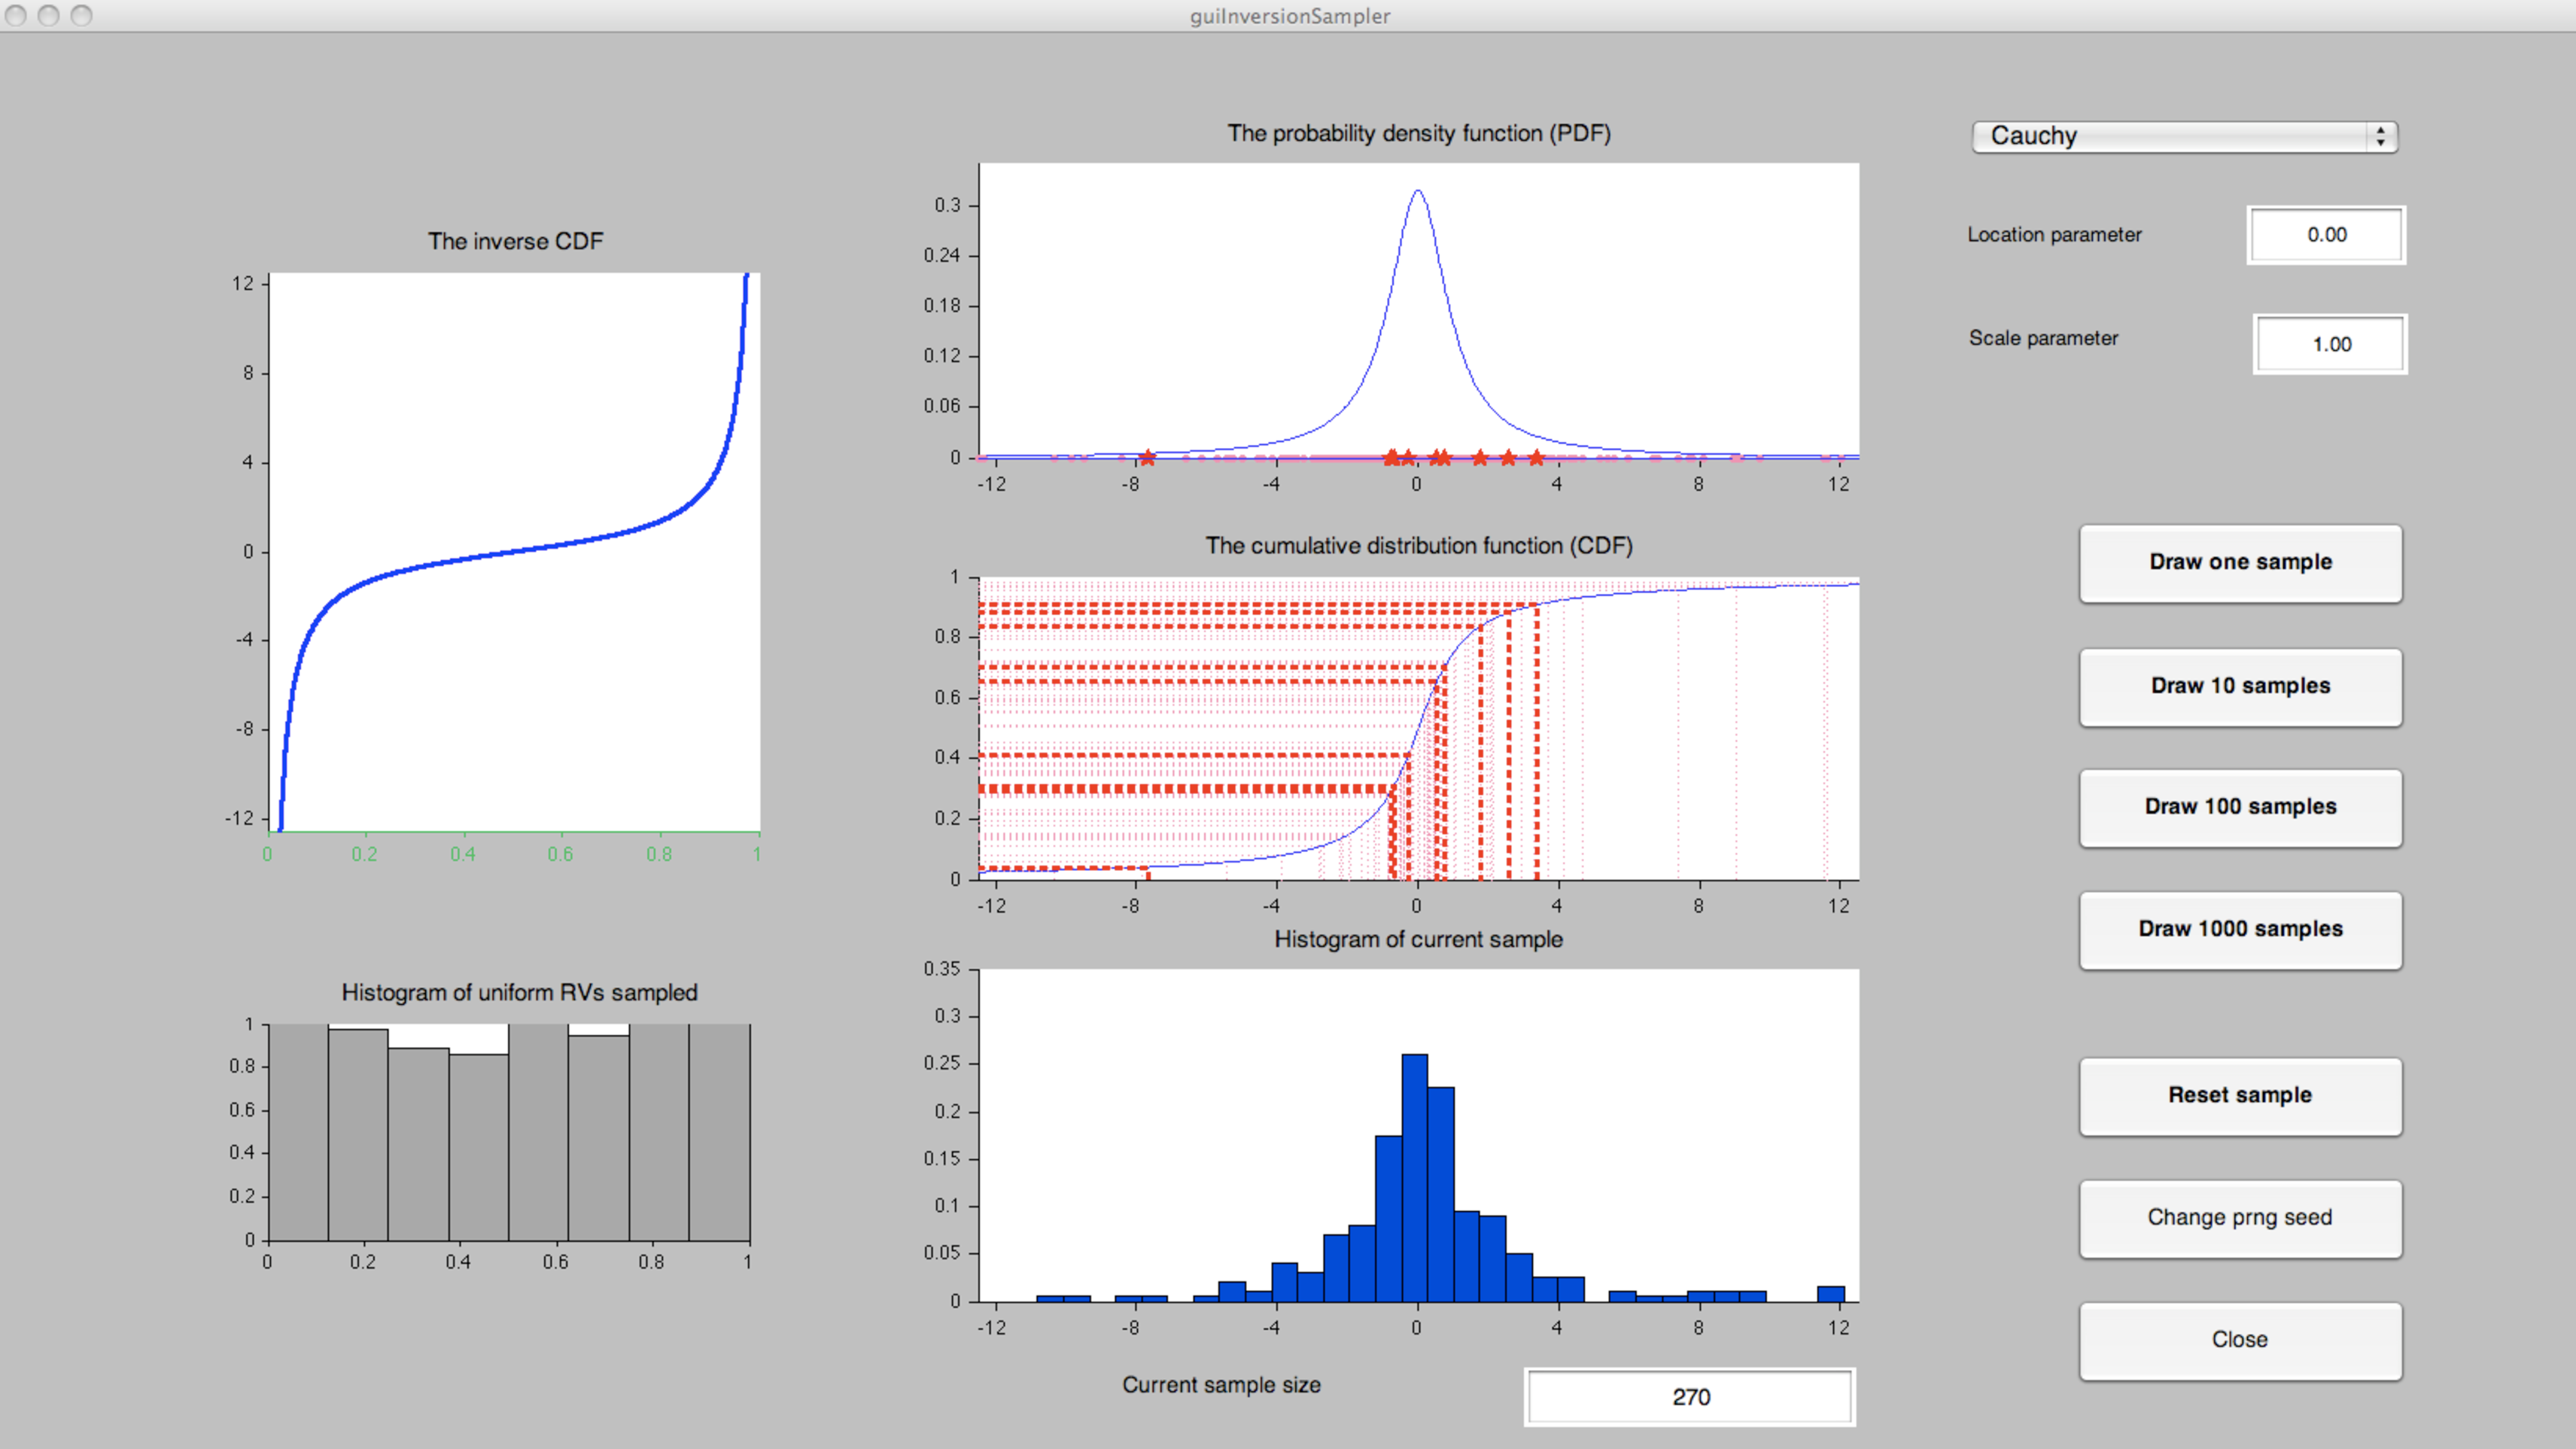
\includegraphics[width=6.50in]{figures/guiInversionSamplerCauchy}}
\end{figure}

\begin{simulation}[$\cauchy$]\label{SIM:StdCauchy}
We can draw $n$ IID samples from the $\cauchy$ RV $X$ by transforming $n$ IID samples from $\uniform(0,1)$ RV $U$ using the inverse DF as follows:
\begin{VrbM}
>> rand('twister',2435567);        % initialise the fundamental sampler
>> u=rand(1,5);			% draw 5 IID samples from Uniform(0,1) RV
>> disp(u);			% display the samples in u
    0.7176    0.6655    0.9405    0.9198    0.2598
>> x=tan(pi * u);     % draw 5 samples from Standard cauchy RV using inverse CDF
>> disp(x);  % display the samples in x
   -1.2272   -1.7470   -0.1892   -0.2575    1.0634
\end{VrbM}
\end{simulation}


\subsection{Inversion Sampler for Discrete Random Variables}\label{S:InvSDiscrete}
Next, consider the problem of {\bf sampling from a random variable $X$ with a discontinuous or discrete DF} using the inversion sampler.  We need to define the inverse more carefully here.
\begin{prop}[Inversion sampler with compact support]
Let the support of the RV $X$ be over some real interval $[a,b]$ and let its inverse DF be defined as follows:
\[
F^{[-1]}(u) := \inf\{ x \in [a,b]: F(x) \geq u, \ 0 \leq u \leq 1 \} \ .
\]
If $U \sim \uniform(0,1)$ then $F^{[-1]}(U)$ has the DF $F$, i.e.~$F^{[-1]}(U) \sim F \sim X$.
\end{prop}
\begin{proof}
The proof is a consequence of the following equalities:
\[
\p(F^{[-1]}(U) \leq x) = \p(U \leq F(x)) = F(x) := \p(X \leq x)
\]
\end{proof}

%\section{Some Simulations of Discrete Random Variables}\label{S:InvSDiscreteRVs}

\begin{simulation}[$\bernoulli(\theta)$]\label{SIM:Bernoulli}
Consider the problem of simulating from a $\bernoulli(\theta)$ RV based on an input from  a $\uniform(0,1)$ RV.  Recall that $\lfloor x \rfloor$ (called the `floor of $x$') is the largest integer that is smaller than or equal to $x$, e.g.~$\lfloor 3.8 \rfloor = 3$.  Using the floor function, we can simulate a $\bernoulli(\theta)$ RV $X$ as follows:
\begin{VrbM}
>>  theta = 0.3;		% set theta = Prob(X=1)
  % return x  -- floor(y) is the largest integer less than or equal to y
>> x = floor(rand + theta)	% rand is the Fundamental Sampler
>> disp(x) % display the outcome of the simulation
     0
>> n=10;  % set the number of IID Bernoulli(theta=0.3) trials you want to simulate
>> x = floor(rand(1,10)+theta); % vectorize the operation
>> disp(x) % display the outcomes of the simulation
     0     0     1     0     0     0     0     0     1     1
\end{VrbM}
\end{simulation}
Again, it is straightforward to do replicate experiments, e.g.~to demonstrate the Central Limit Theorem for a sequence of $n$ IID $\bernoulli(\theta)$ trials.
\begin{VrbM}
>> % a demonstration of Central Limit Theorem --
>> % the sample mean of a sequence of n IID Bernoulli(theta) RVs is Gaussian(theta,theta(1-theta)/n)
>> theta=0.5; Reps=10000; n=10; hist(sum(floor(rand(n,Reps)+theta))/n)
>> theta=0.5; Reps=10000; n=100; hist(sum(floor(rand(n,Reps)+theta))/n,20)
>> theta=0.5; Reps=10000; n=1000; hist(sum(floor(rand(n,Reps)+theta))/n,30)
\end{VrbM}

Recall the $\pointmass(\theta)$ RV. Formally, we can simulate from it trivially as follows.
\begin{simulation}[$\pointmass(\theta)$]\label{SIM:PointMass}
Let us simulate a sample from the $\pointmass(\theta)$ RV $X$.  Since this RV produces the same realisation $\theta$ we can implement it via the following M-file:

\VrbMf[label=Sim1PointMass.m]{scripts/Sim1PointMass.m}
Here is call to the function.
\begin{VrbM}
>> Sim1PointMass(rand(),2)
ans =     2
>> % % we can use arrayfun to apply Sim1Pointmass to any array of Uniform(0,1) samples
>> arrayfun(@(u)(Sim1PointMass(u,17)),rand(2,10))
ans =
    17    17    17    17    17    17    17    17    17    17
    17    17    17    17    17    17    17    17    17    17
\end{VrbM}
Note that it is not necessary to have input IID samples from $\uniform(0,1)$ RV via {\tt rand} in order to draw samples from the $\pointmass(\theta)$ RV.  For instance, an input matrix of zeros can do the job:
\begin{VrbM}
>> arrayfun(@(u)(Sim1PointMass(u,17)),zeros(2,8))
ans =
    17    17    17    17    17    17    17    17
    17    17    17    17    17    17    17    17
\end{VrbM}
\end{simulation}

Next we simulate from $\demoivre(\theta_1,\theta_2,\ldots,\theta_k)$ RV $X$ of Model~\ref{M:demoivre} via its inverse DF $$F^{[-1]}: [0,1] \rightarrow [k] := \{1,2,\ldots,k\} \ ,$$ given by:
\begin{equation}\label{E:deMoivreInverseDF}
F^{[-1]}(u;\theta_1,\theta_2,\ldots,\theta_k) =
\begin{cases}
1 & \quad \text{if $0 \leq u < \theta_1$}\\
2 & \quad \text{if $\theta_1 \leq u < \theta_1+\theta_2$} \\
3 & \quad \text{if $\theta_1+\theta_2 \leq u < \theta_1+\theta_2+\theta_3$} \\
\vdots & \\
k & \quad \text{if $\theta_1+\theta_2+\cdots+\theta_{k-1} \leq u < 1$} \\
\end{cases}
\end{equation}
When $k=2$ in the $\demoivre(\theta_1,\theta_2)$ model, we have an RV that is similar to the $\bernoulli(p=\theta_1)$ RV.  The DF $F$ and its inverse $F^{[-1]}$ for a specific $\theta_1=0.3$ are depicted in \hyperref[F:InvSamk2]{Figure \ref*{F:InvSamk2}}.

\begin{figure}[htpb]
\caption{The DF $F(x;0.3,0.7)$ of the $\demoivre(0.3,0.7)$ RV and its inverse $F^{[-1]}(u;0.3,0.7)$. \label{F:InvSamk2}}
\centering   \makebox{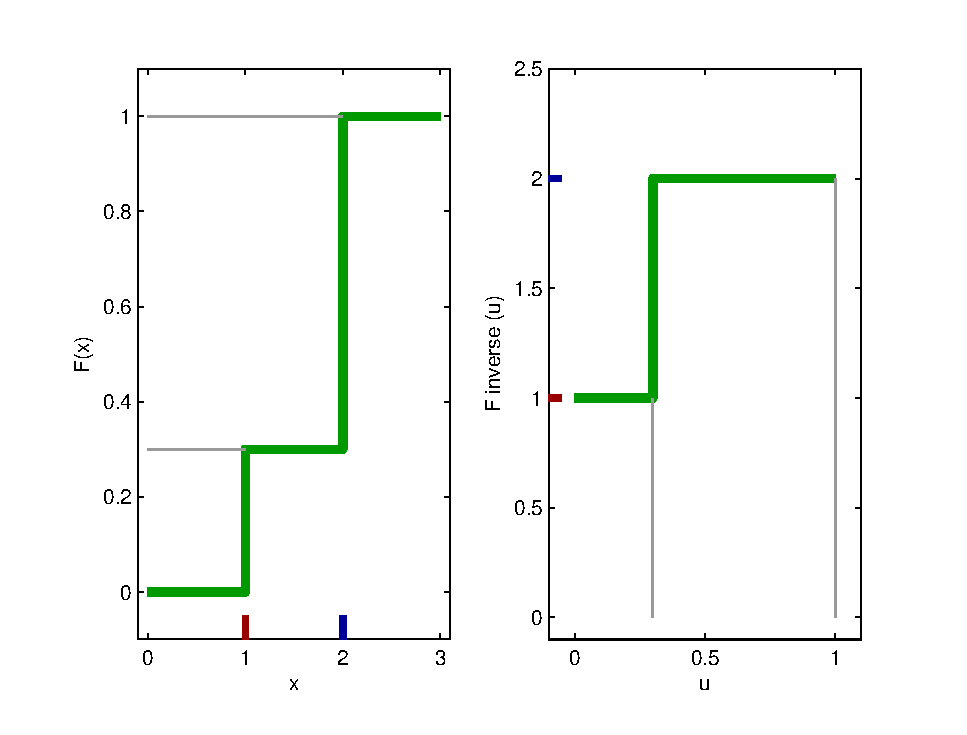
\includegraphics[width=10cm]{figures/plotInvSamk2R}}
\end{figure}

First we simulate from an equi-probable special case of the $\demoivre(\theta_1,\theta_2,\ldots,\theta_k)$ RV, with $\theta_1=\theta_2=\cdots=\theta_k=1/k$.
\begin{simulation}[$\demoivre(1/k,1/k,\ldots,1/k)$]\label{SIM:deMoivreEqui}
The equi-probable $de~Moivre(1/k,1/k,\ldots,1/k)$ RV $X$ with a discrete uniform distribution over $[k] = \{1,2,\ldots k\}$ can be efficiently sampled using the ceiling function.  Recall that $\lceil y \rceil$ is the smallest integer larger than or equal to $y$, eg.~$\lceil 13.1 \rceil = 14$.  \hyperref[A:SimdeMoivreEqui]{Algorithm~\ref*{A:SimdeMoivreEqui}} produces samples from the $de~Moivre(1/k,1/k,\ldots,1/k)$ RV $X$.

\begin{algorithm}[h]
\caption{ Inversion Sampler  for $\demoivre(1/k,1/k,\ldots,1/k)$ RV}
\label{A:SimdeMoivreEqui}
\begin{algorithmic}[1]
\STATE {
{\it input:}
\begin{enumerate}
\item $k$ in $\demoivre(1/k,1/k,\ldots,1/k)$ RV $X$
\item $u \sim \uniform(0,1)$
\end{enumerate}
}
\STATE {\it output:} a sample from $X$
\STATE {{\it return:} $x \gets \lceil k u \rceil $}
\end{algorithmic}
\end{algorithm}

The M-file implementing \hyperref[A:SimdeMoivreEqui]{Algorithm~\ref*{A:SimdeMoivreEqui}} is:
 \VrbMf[label=SimdeMoivreEqui.m]{scripts/SimdeMoivreEqui.m}
Let us use the function {\tt SimdeMoivreEqui} to draw five samples from a fair seven-faced cylindrical dice.
\begin{VrbM}
>> k=7; % number of faces of the fair dice
>> n=5; % number of trials
>> rand('twister',78657); % initialise the fundamental sampler
>> u=rand(1,n); % draw n samples from Uniform(0,1)
>> % inverse transform samples from Uniform(0,1) to samples
>> % from de Moivre(1/7,1/7,1/7,1/7,1/7,1/7,1/7)
>> outcomes=SimdeMoivreEqui(u,k); % save the outcomes in an array
>> disp(outcomes);
     6     5     5     5     2
\end{VrbM}
\end{simulation}

Now, let us consider the more general problem of implementing a sampler for an arbitrary but specified $\demoivre(\theta_1,\theta_2,\ldots,\theta_k)$ RV.  That is, the values of $\theta_i$ need not be equal to $1/k$.
\begin{simulation}[$\demoivre(\theta_1,\theta_2,\ldots,\theta_k)$]\label{SIM:deMoivre}
We can generate samples from a $\demoivre(\theta_1,\theta_2,\ldots,\theta_k)$ RV $X$ when $(\theta_1,\theta_2,\ldots,\theta_k)$ are specifiable as an input vector via the following algorithm.

\begin{algorithm}
\caption{Inversion Sampler for $\demoivre(\theta_1,\theta_2,\ldots,\theta_k)$ RV $X$}
\label{A:SimdeMoivre}
\begin{algorithmic}[1]
\STATE {
{\it input:}
\begin{enumerate}
\item parameter vector $(\theta_1,\theta_2,\ldots,\theta_k)$ of $\demoivre(\theta_1,\theta_2,\ldots,\theta_k)$ RV $X$.
\item $u \sim \uniform(0,1)$
\end{enumerate}
}
\STATE {\it output:} a sample from $X$
\STATE {\it initialise:}  $F \gets \theta_1$, $i \gets 1$
\WHILE{$u > F$}
\STATE $i \gets i+1$
\STATE $F \gets F+\theta_{i}$
\ENDWHILE
\STATE {\it return:} $x \gets i$
\end{algorithmic}
\end{algorithm}

The M-file implementing \hyperref[A:SimdeMoivre]{Algorithm~\ref*{A:SimdeMoivre}} is:
 \VrbMf[label=SimdeMoivreOnce.m]{scripts/SimdeMoivreOnce.m}
Let us use the function {\tt deMoivreEqui} to draw five samples from a fair seven-faced dice.
\begin{VrbM}
>> k=7; % number of faces of the fair dice
>> n=5; % number of trials
>> rand('twister',78657); % initialise the fundamental sampler
>> Us=rand(1,n); % draw n samples from Uniform(0,1)
>> disp(Us);
    0.8330    0.6819    0.6468    0.6674    0.2577
>> % inverse transform samples from Uniform(0,1) to samples
>> % from de Moivre(1/7,1/7,1/7,1/7,1/7,1/7,1/7)
>> f=[1/7 1/7 1/7 1/7 1/7 1/7 1/7];
>> disp(f);
    0.1429    0.1429    0.1429    0.1429    0.1429    0.1429    0.1429
>> % use funarray to apply function-handled SimdeMoivreOnce to
>> % each element of array Us and save it in array outcomes2
>> outcomes2=arrayfun(@(u)(SimdeMoivreOnce(u,f)),Us);
>> disp(outcomes2);
     6     5     5     5     2
>> disp(SimdeMoivreEqui(u,k)); % same result using the previous algorithm
     6     5     5     5     2
\end{VrbM}
Clearly, \hyperref[A:SimdeMoivre]{Algorithm~\ref*{A:SimdeMoivre}} may be used to sample from any $\demoivre(\theta_1,\ldots,\theta_k)$ RV $X$.  We demostrate this by producing five samples from a randomly generated PMF {\tt f2}.
\begin{VrbM}
>> rand('twister',1777); % initialise the fundamental sampler
>> f2=rand(1,10); % create an arbitrary array
>> f2=f2/sum(f2); % normalize to make a probability mass function
>> disp(f2); % display the weights of our 10-faced die
    0.0073    0.0188    0.1515    0.1311    0.1760    0.1121    ...
    0.1718    0.1213    0.0377    0.0723
>> disp(sum(f2)); % the weights sum to 1
    1.0000
>> disp(arrayfun(@(u)(SimdeMoivreOnce(u,f2)),rand(5,5))) % the samples from f2 are
     4     3     4     7     3
     6     7     4     5     3
     5     8     7    10     6
     2     3     5     7     7
     6     5     9     5     7
\end{VrbM}
\end{simulation}

Note that the principal work here is the sequential search, in which the mean number of comparisons until success is:
\[
1 \theta_1 + 2 \theta_2 + 3 \theta_3 + \ldots + k \theta_k = \sum_{i=1}^k{ i \theta_i}
\]
For the $\demoivre(1/k,1/k,\ldots,1/k)$ RV, the right-hand side of the above expression is:
\[
\sum_{i=1}^k{ i \frac{1}{k}} = \frac{1}{k} \sum_{i=1}^k{ i} = \frac{1}{k} \frac{k(k+1)}{2} = \frac{k+1}{2} \ ,
\]
indicating that the average-case efficiency is linear in $k$.  This linear dependence on $k$ is denoted by $O(k)$.  In other words, as the number of faces $k$ increases, one has to work linearly harder to get samples from $\demoivre(1/k,1/k,\ldots,1/k)$ RV using \hyperref[A:SimdeMoivre]{Algorithm \ref*{A:SimdeMoivre}}.  Using the simpler \hyperref[A:SimdeMoivreEqui]{Algorithm \ref*{A:SimdeMoivreEqui}}, which exploits the fact that all values of $\theta_i$  are equal, we generated samples in constant time, which is denoted by $O(1)$.
%}%end remove

%\remove{
\begin{simulation}[$\geometric(\theta)$]\label{SIM:Geometric}
We can simulate a sample $x$ from a $\geometric(\theta)$ RV $X$ using the following simple algorithm:
\[
x \gets \lfloor \log(u) / \log(1-\theta) \rfloor, \qquad \text{where, } \ u \sim \uniform(0,1) \ .
\]
To verify that the above procedure is valid, note that:
\begin{align}
\lfloor \log(U) / \log(1-\theta) \rfloor = x
& \iff x \leq  \log(U) / \log(1-\theta) < x+1 \notag \\
& \iff x \leq  \log_{1-\theta}(U) < x+1 \notag \\
& \iff (1-\theta)^x \geq U > (1-\theta) ^{x+1} \notag
\end{align}
The inequalities are reversed since the base being exponentiated is $1-\theta \leq 1$.  The uniform event $(1-\theta)^x \geq U > (1-\theta) ^{x+1}$ happens with the desired probability:
$$(1-\theta) ^{x}-(1-\theta) ^{x+1} = (1-\theta) ^{x}(1-(1-\theta)) = \theta (1-\theta) ^{x} =: f(x;\theta), \quad X \sim \geometric(\theta) \ .$$

We implement the sampler to generate samples from $\geometric(\theta)$ RV with $\theta=0.5$, for instance:
\begin{VrbM}
>> theta=0.5; u=rand(); % choose some theta and uniform(0,1) variate
>> % Simulate from a Geomertic(theta) RV
>> floor(log (u) / log (1 - theta))
ans =     0
>> floor(log ( rand(1,10) ) / log (1 - 0.5)) % theta=0.5, 10 samples
ans =     0     0     1     0     2     1     0     0     0     0
\end{VrbM}
\end{simulation}

\begin{labwork}[PMF versus relative frequency histogram of simulated $\geometric(\theta)$ RV]\label{LW:RelFreqHistForGeomSims}
It is a good idea to make a relative frequency histogram of a simulation algorithm and compare that to the PDF of the discrete RV we are simulating from.  We use the following script to create \hyperref[F:PlotPdfSimHistGeomthetaHalf]{Figure \ref*{F:PlotPdfSimHistGeomthetaHalf}}:
\VrbMf[label=PlotPdfSimGeometric.m]{scripts/PlotPdfSimGeometric.m}
\end{labwork}

Let us simulate from the $\binomial(n,\theta)$ RV of Model~\ref{M:binomial}. %TODO hyperref.
%\remove{
\begin{labwork}[Binomial coefficient]\label{LW:BinomialPdf}
The \Matlab function {\tt BinomialCoefficient} can be used to compute:
\[
\binom{n}{x} =  \frac{n !}{x! (n-x)!} = \frac{n(n-1)(n-2)\ldots(n-x+1)}{x(x-1)(x-2)\cdots (2)(1)} = \frac{\prod_{i=(n-x+1)}^n i}{\prod_{i=2}^x} \ ,
\]
with the following M-file:
\VrbMf[label=BinomialCoefficient.m]{scripts/BinomialCoefficient.m}
and call {\tt BinomialCoefficient} in the function {\tt BinomialPdf} to compute the PDF $f(x;n,\theta)$ of the $\binomial(n,\theta)$ RV $X$ as follows:
\VrbMf[label=BinomialPdf.m]{scripts/BinomialPdf.m}
For example, we can compute the desired PDF for an array of samples {\tt x} from $\binomial(8,0.5)$ RV $X$, as follows:
\begin{VrbM}
>> x=0:1:8
x =     0     1     2     3     4     5     6     7     8
>> BinomialPdf(x,8,0.5)
ans =    0.0039    0.0312    0.1094    0.2188    0.2734    0.2188    0.1094    0.0312    0.0039
\end{VrbM}
\end{labwork}

\begin{simulation}[$\binomial(n,\theta)$ as $\sum_{i=1}^n \bernoulli(\theta)$]\label{SIM:BinomialFromBernoulliSum}
Since the $\binomial(n,\theta)$ RV $X$ is the sum of $n$ IID $\bernoulli(\theta)$ RVs we can also simulate from $X$ by first simulating $n$ IID $\bernoulli(\theta)$ RVs and then adding them up as follows:
\begin{VrbM}
>> rand('twister',17678);
>> theta=0.5; % give some desired theta value, say 0.5
>> n=5; % give the parameter n for Binomial(n,theta) RV X, say n=5
>> xis=floor(rand(1,n)+theta) % produce n IID samples from Bernoulli(theta=0.5) RVs X1,X2,...Xn
xis =     1     1     0     0     0
>> x=sum(xis) % sum up the xis to get a sample from Binomial(n=5,theta=0.5) RV X
x =     2
\end{VrbM}
It is straightforward to produce more than one sample from $X$ by exploiting the column-wise summing property of \Matlab's {\tt sum} function when applied to a two-dimensional array:
\begin{VrbM}
>> rand('twister',17);
>> theta=0.25; % give some desired theta value, say 0.25 this time
>> n=3; % give the parameter n for Binomial(n,theta) RV X, say n=3 this time
>> xis10 = floor(rand(n,10)+theta) % produce an n by 10 array of IID samples from Bernoulli(theta=0.25) RVs
xis10 =
     0     0     0     0     1     0     0     0     0     0
     0     1     0     1     1     0     0     0     0     0
     0     0     0     0     0     0     0     1     0     0
>> x=sum(xis10) % sum up the array column-wise to get 10 samples from Binomial(n=3,theta=0.25) RV X
x =     0     1     0     1     2     0     0     1     0     0
\end{VrbM}
\end{simulation}

In \hyperref[SIM:BinomialFromBernoulliSum]{Simulation \ref*{SIM:BinomialFromBernoulliSum}}, the number of IID $\bernoulli(\theta)$ RVs needed to simulate one sample from the $\binomial(n,\theta)$ RV is exactly $n$.  Thus, as $n$ increases, the amount of time needed to simulate from $\binomial(n,\theta)$ is $O(n)$, i.e.~linear in $n$.  We can simulate more efficiently by exploiting a simple relationship between the $\geometric(\theta)$ RV and the $\binomial(n,\theta)$ RV.


The $\binomial(n,\theta)$ RV $X$ is related to the IID $\geometric(\theta)$ RV $Y_1,Y_2,\ldots$: $X$ is the number of successful $\bernoulli(\theta)$ outcomes (outcome is $1$) that occur in a total of $n$ $\bernoulli(\theta)$ trials, with the number of trials between consecutive successes distributed according to IID $\geometric(\theta)$ RV.
\begin{simulation}[$\binomial(\theta)$ from IID $\geometric(\theta)$ RVs]\label{SIM:BinomialFromGeoms}
By this principle, we can simulate from the $\binomial(\theta)$ $X$ by {\sf Step 1}: generating IID $\geometric(\theta)$ RVs $Y_1,Y_2,\ldots$, {\sf Step 2}: stopping as soon as $\sum_{i=1}^k (Y_i+1) > n$ and {\sf Step 3:} setting $x \gets k-1$.

We implement the above algorithm via the following M-file:
\VrbMf[label=Sim1BinomByGeoms.m]{scripts/Sim1BinomByGeoms.m}
Here is a call to simulate $12$ samples from $\binomial(n=10,\theta=0.5)$ RV:
\begin{VrbM}
>> theta=0.5; % declare theta
>> n=10; % say n=10
>> SampleSize=12;% say you want to simulate 12 samples
>> rand('twister',10001) % seed the fundamental sampler
>> Samples=arrayfun(@(T)Sim1BinomByGeoms(n,T),theta*ones(1,SampleSize))
Samples =     7     5     8     8     4     1     4     8     2     4     6     5
\end{VrbM}
\hyperref[F:PlotPdfSim10000HistBinomByGeomsn10thetaHalf]{Figure \ref*{F:PlotPdfSim10000HistBinomByGeomsn10thetaHalf}} depicts a comparison of the PDF of $\binomial(n=10,\theta=0.5)$ RV and a relative frequency histogram based on $100,000$ simulations from it.
\end{simulation}
%}% end remove

%\remove{
Let us simulate from the $\poisson(\lambda)$ RV of Model~\ref{M:Poisson} as shown in Figure~\ref{F:PlotPdfSim1000HistPoiss10}. % TODO href

\begin{simulation}[$\poisson(\lambda)$ from IID $\exponential(\lambda)$ RVs]\label{SIM:Poisson}
By this principle, we can simulate from the $\poisson(\lambda)$ $X$ by {\sf Step 1}: generating IID $\exponential(\lambda)$ RVs $Y_1,Y_2,\ldots$, {\sf Step 2}: stopping as soon as $\sum_{i=1}^k Y_i \geq 1$ and {\sf Step 3:} setting $x \gets k-1$.

We implement the above algorithm via the following M-file:
\VrbMf[label=Sim1Poisson.m]{scripts/Sim1Poisson.m}
Here is a call to simulate 10 samples from $\poisson(\lambda=10.0)$ and $\poisson(\lambda=0.1)$ RVs:
\begin{VrbM}
>> arrayfun(@(lambda)Sim1Poisson(lambda),10.0*ones(1,10)) % lambda=10.0
ans =    14     7    10    13    11     3     6     5     8     5
>> arrayfun(@(lambda)Sim1Poisson(lambda),0.1*ones(1,10)) % lambda=0.1
ans =     2     0     0     0     0     0     0     0     0     0
\end{VrbM}
\hyperref[F:PlotPdfSim1000HistPoiss10]{Figure \ref*{F:PlotPdfSim1000HistPoiss10}} depicts a comparison of the PDF of $\poisson(\lambda=10)$ RV and a relative frequency histogram based on 1000 simulations from it.
\end{simulation}

Simulating from a $\poisson(\lambda)$ RV is also a special case of simulating from the following more general RV.
\begin{model}[$GD(\theta_0,\theta_1,\ldots)$]
We say $X$ is a $\generaldiscrete(\theta_0,\theta_1,\ldots)$ or $\GD(\theta_0,\theta_1,\ldots)$ RV over the countable discrete state space $\Zz_+ := \{0,1,2,\ldots\}$ with parameters $(\theta_0,\theta_1,\ldots)$ if the PMF of $X$ is defined as follows:
\[
f(X=x; \theta_0,\theta_1,\ldots) =
\begin{cases}
0, & if \quad x \notin  \{0,1,2,\ldots\} \\
 \theta_0, & if \quad x=0 \\
 \theta_1, & if \quad x=1 \\
\vdots & \\
\end{cases}
\]
\hyperref[A:InvSGenDisc]{Algorithm \ref*{A:InvSGenDisc}} allows us to simulate from any member of the class of non-negative discrete RVs as specified by the probabilities $(\theta_0,\theta_1,\ldots)$.  When an RV $X$ takes  values in another countable set $\Xz \neq \Zz_+$, then we can still use the above algorithm provided we have a one-to-one and onto mapping $D(i)=x: \Zz_+ \to \Xz$ that allows us to think of $\left(0,1,2,\ldots\right)$ as indices of an array $D$ giving $\Xz = \left(D(0), D(1), \ldots \right)$.
\end{model}

\begin{algorithm}
\caption{Inversion Sampler for $GD(\theta_0,\theta_1,\ldots)$ RV $X$}
\label{A:InvSGenDisc}
\begin{algorithmic}[1]
\STATE {
{\it input:}
\begin{enumerate}
\item $\theta_0$ and $\{ C(i)  = \theta_{i}/\theta_{i-1} \}$ for any $i \in \{1,2,3,\ldots\}$.
\item $u \sim \uniform(0,1)$
\end{enumerate}
}
\STATE {\it output:} a sample from $X$
\STATE {\it initialise:} $p \gets \theta_0$, $q \gets \theta_0$, $i \gets 0$
\WHILE{$u > q$}
\STATE $i \gets i+1$, $p \gets p \ C(i)$, $q \gets q+p$
\ENDWHILE
\STATE {\it return:} $x = i$
\end{algorithmic}
\end{algorithm}

%\begin{classwork}
%What is the algorithm's efficiency when applied to the $\demoivre(\theta_1,\theta_2,\ldots,\theta_k)$ ?
%Worst-case and average-case efficiency ?
%\vspace{5cm}
%\end{classwork}


\begin{simulation}[$\binomial(n,\theta)$]
To simulate from a $\binomial(n,\theta)$ RV $X$, we can use \hyperref[A:InvSGenDisc]{Algorithm \ref*{A:InvSGenDisc}} with:
\[
\theta_0=(1-\theta)^n, \qquad C(x+1)=\frac{\theta(n-x)}{(1-\theta)(x+1)}, \qquad \text{Mean Efficiency: $O(1+n\theta)$} \ .
\]
\end{simulation}
Similarly, with the appropriate $\theta_0$ and $C(x+1)$, we can also simulate from the $\geometric(\theta)$ and $\poisson(\lambda)$ RVs.

\begin{labwork}This is a challenging exercise for the student who is finding the other Labworks too easy. So those who are novice to \Matlab may skip this Labwork.
\begin{enumerate}
\item Implement \hyperref[A:InvSGenDisc]{Algorithm \ref*{A:InvSGenDisc}} via a function named {\tt MyGenDiscInvSampler} in {\tt MATLAB}.  Hand in the {\tt M-file} named {\tt MyGenDiscInvSampler.m} giving detailed comments explaining your understanding of each step of the code.  [Hint: $C(i)$ should be implemented as a function (use function handles via {\tt @}) that can be passed as a parameter to the function {\tt MyGenDiscInvSampler}].
\item Show that your code works for drawing samples from a $\binomial(n,p)$ RV by doing the following:
\begin{enumerate}
\item Seed the fundamental sampler by your Student ID (if your ID is {\tt 11424620} then type {\tt rand('twister', 11424620);})
\item Draw 100 samples from the $\binomial(n=20,p=0.5)$ RV and report the results in an $2 \times 2$ table with column headings {\tt x} and {No. of observations}.  [Hint: the inputs $\theta_0$ and $C(i)$ for the $\binomial(n,p)$ RV is given above].
\end{enumerate}
\item Show that your code works for drawing samples from a $\geometric(p)$ RV by doing the following:
\begin{enumerate}
\item Seed the fundamental sampler by your Student ID.
\item Set the variable {\tt Mytheta=rand}.
\item Draw 100 samples from the $\geometric({\tt Mytheta})$ RV and report the sample mean.  [Note: the inputs $\theta_0$ and $C(i)$ for the $\geometric(\theta)$ RV should be derived and the workings shown].
\end{enumerate}
\end{enumerate}
\end{labwork}

\subsection{von Neumann Rejection Sampler (RS)}\label{S:RS}
Rejection sampling [John von Neumann, 1947, in {\it Stanislaw Ulam 1909-1984}, a special issue of Los Alamos Science, Los Alamos National Lab., 1987, p.~135-136] is a Monte Carlo method to draw independent
samples from a target RV $X$ with probability density $f(x)$, where $x \in \Xz \subset \Rz^k$.  Typically, the target density $f$ is only known up to a constant and therefore the (normalised) density $f$ itself may be unknown and it  is difficult to generate samples directly from $X$.

Suppose we have another density or mass function $g$ for which the following are true:
\begin{asparaenum}[(a)]
\item	we can generate random variables from $g$;
\item	the support of $g$ contains the support of $f$, i.e.~$\Yz \supset \Xz$;
\item	a constant $a > 1$ exists, such that:
\begin{equation}
f(x)\leq ag(x).
\end{equation}
for any $x\in \Xz$, the support of $X$.  Then $x$ can be generated from Algorithm \ref*{A:RS}.
\end{asparaenum}

\begin{algorithm}
\caption{Rejection Sampler (RS) of von Neumann}
\label{A:RS}
\begin{algorithmic}[1]
\STATE {
{\it input:}
\begin{itemize}
\item[(1)] a target density $f(x)$,
\item[(2)] a proposal density $g(x)$ satisfying (a), (b) and (c) above.
\end{itemize}
}
\STATE {\it output:} a sample $x$ from RV $X$ with density $f$

\REPEAT
\STATE Generate $y \sim g$ and $u \sim \uniform(0,1)$
\UNTIL{$u \leq \frac{f(y)}{a g(y)}$}
\STATE {\it return:} $x \gets y$
\end{algorithmic}
\end{algorithm}

\begin{prop}[Fundamental Theorem of Simulation]  The von Neumann rejection sampler of Algorithm \ref*{A:RS} produces a sample $x$ from the random variable $X$ with density $f(x)$.
\begin{proof}
We shall prove the result for the continuous case. For any real number $t$:

\begin{eqnarray*}
F(t) &= \p(X \leq t) = \p\left(Y \leq t  \, | \, U \leq\frac{f(Y)}{ag(Y)} \right)
=\frac{\p\left(Y \leq t, U \leq\frac{f(Y)}{ag(Y)} \right)}{\p\left(U \leq\frac{f(Y)}{ag(Y)}\right)}\\
&=\frac{\int^t_{-\infty}\left(\int^{f(y)/ag(y)}_0 1 du\right)g(y)dy}{\int^{\infty}_{-\infty}\left(\int^{f(y)/ag(y)}_0 1 du\right)g(y)dy}
=\frac{\int^t_{-\infty}\left(\frac{f(y)}{ag(y)} \right)g(y)dy}{\int^{\infty}_{-\infty}\left(\frac{f(y)}{ag(y)} \right)g(y)dy}\\
&=\int^t_{-\infty}f(y)dy
\end{eqnarray*}
\end{proof}
\end{prop}

\begin{labwork}[Rejection Sampler Demo]\label{LW:guiRejectionsNormal01}
Let us understand the rejection sampler by calling the interactive visual cognitive tool:
\begin{VrbM}
>> guiRejections
\end{VrbM}
The M-file {\tt guiRejections.m} will bring a graphical user interface (GUI) as shown in \hyperref[F:guiRejectionsNormal01]{Figure \ref*{F:guiRejectionsNormal01}}.  Try various buttons and see how the output changes with explanations.  Try switching the ``Target distribution'' to ``Mywavy4'' and generate several rejection samples and see the density histogram of the accumulating samples.
\end{labwork}

\begin{figure}[htpb]
\caption{Visual Cognitive Tool GUI: Rejection Sampling from $X \sim \normal(0,1)$ with PDF $f$ based on proposals from $Y \sim \laplace(1)$ with PDF $g$.\label{F:guiRejectionsNormal01}}
\centering   \makebox{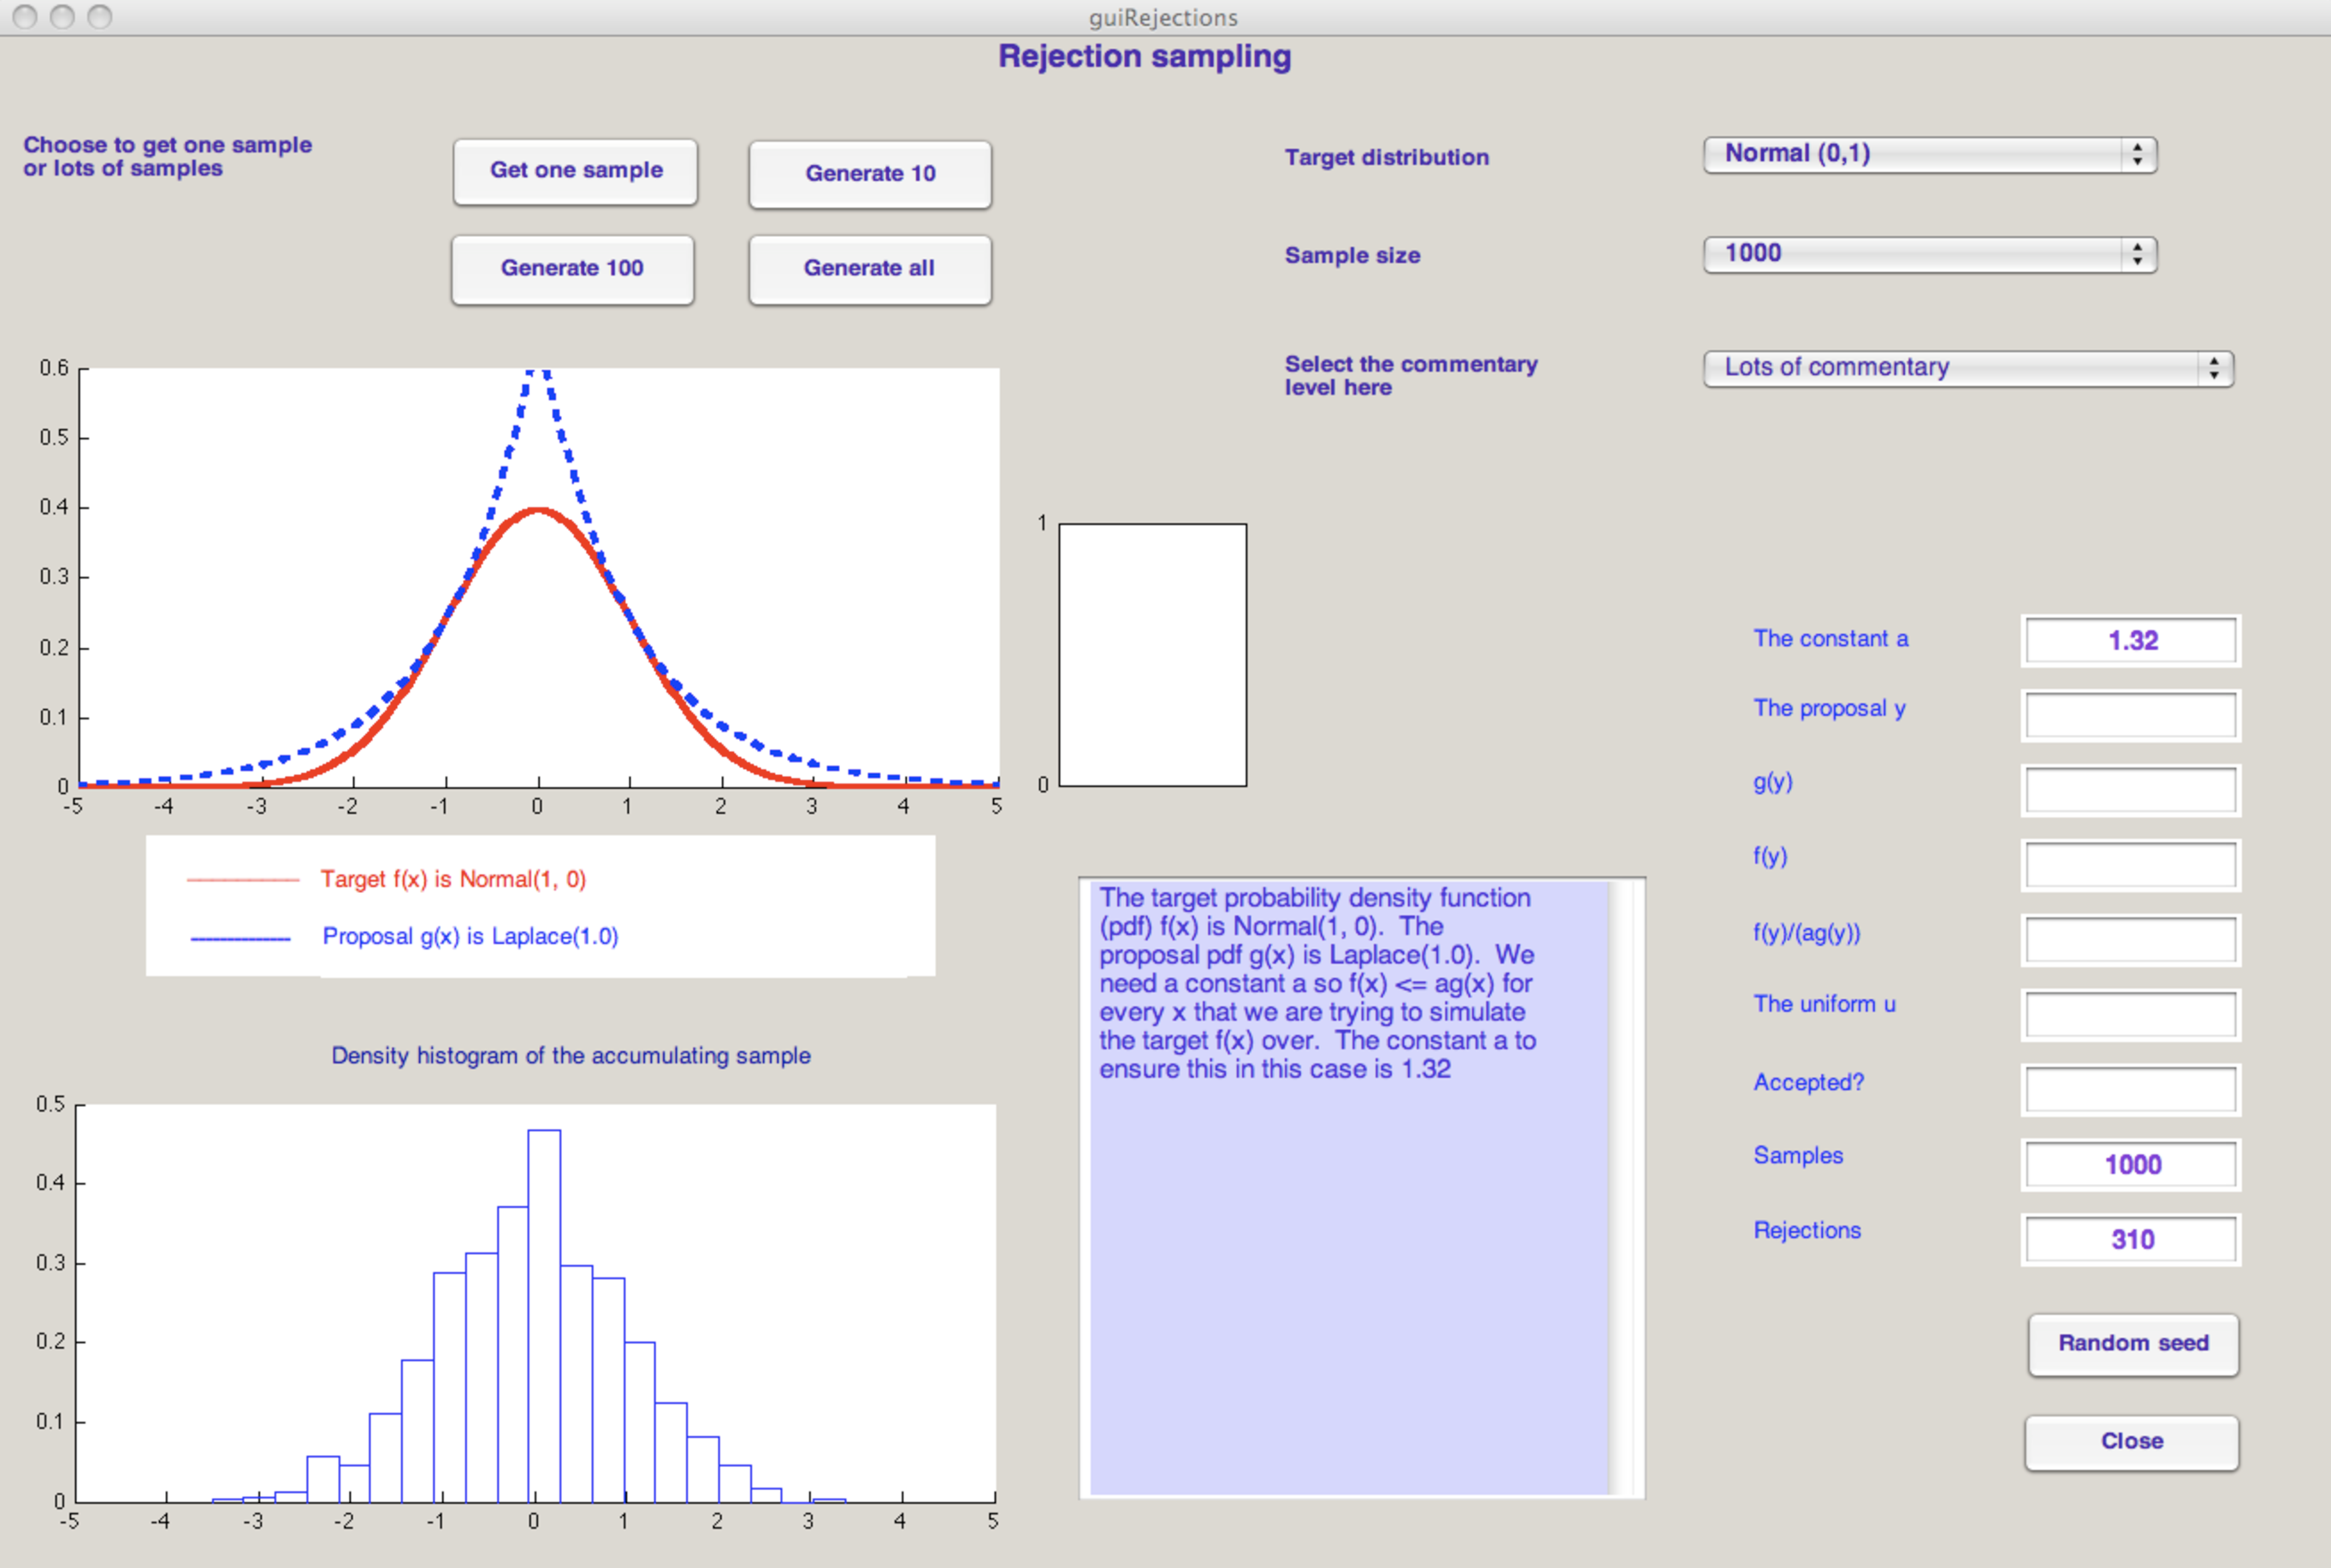
\includegraphics[width=5.50in]{figures/guiRejectionsNormal01}}
\end{figure}


%\subsection{\exmpl ({\tt rejection\_normal\_laplacian.m})}
% % Dominic's Demo needs Stats Toolbox
\begin{simulation}[Rejection Sampling $\normal(0,1)$ with $\laplace(1)$ proposals]\label{SIM:Normal01FromLaplace}
Suppose we wish to generate from $X \sim \normal(0, 1)$. Consider using the rejection sampler with proposals from $Y \sim \laplace(1)$ (using inversion sampler of \hyperref[SIM:Laplace]{Simulation \ref*{SIM:Laplace}}). The support of both RVs is $(-\infty,\infty)$. Next:
$$f(x)=\frac{1}{\sqrt{2\pi}}\exp\left(-\frac{x^2}{2}\right) \textrm{ and } g(x)=\frac{1}{2}\exp(-|x|)$$
and therefore:
$$\frac{f(x)}{g(x)}=\sqrt{\frac{2}{\pi}}\exp\left(|x|-\frac{x^2}{2}\right)\leq \sqrt{\frac{2}{\pi}}\exp\left(\frac{1}{2}\right) = a \approx 1.3155 \ .$$
Hence, we can use the rejection method with:
$$
\frac{f(y)}{a g(y)} = \frac{f(y)}{g(y)} \frac{1}{a} = \sqrt{\frac{2}{\pi}}\exp\left(|y|-\frac{y^2}{2}\right) \frac{1}{\sqrt{\frac{2}{\pi}}\exp\left(\frac{1}{2}\right)  } = \exp\left(|y|-\frac{y^2}{2} - \frac{1}{2} \right)
$$
%\includegraphics

Let us implement a rejection sampler as a function in the M-file {\tt RejectionNormalLaplace.m} by reusing the function in {\tt LaplaceInvCDF.m}.
\VrbMf[label=RejectionNormalLaplace.m]{scripts/RejectionNormalLaplace.m}
We may obtain a large number of samples an plot them as a histogram using the following commands:
\begin{VrbM}
>> % use funarray to convert 1000 zeros into samples from the Normal(0,1)
>> y=arrayfun(@(x)(RejectionNormalLaplace()),zeros(1,1000));
>> hist(y,20) % histogram with 20 bins
\end{VrbM}
\end{simulation}

\begin{figure}[htpb]
\caption{Rejection Sampling from $X \sim \normal(0,1)$ with PDF $f$ based on  100 proposals from $Y \sim \laplace(1)$ with PDF $g$.\label{F:RSNormalLaplace}}
\centering   \makebox{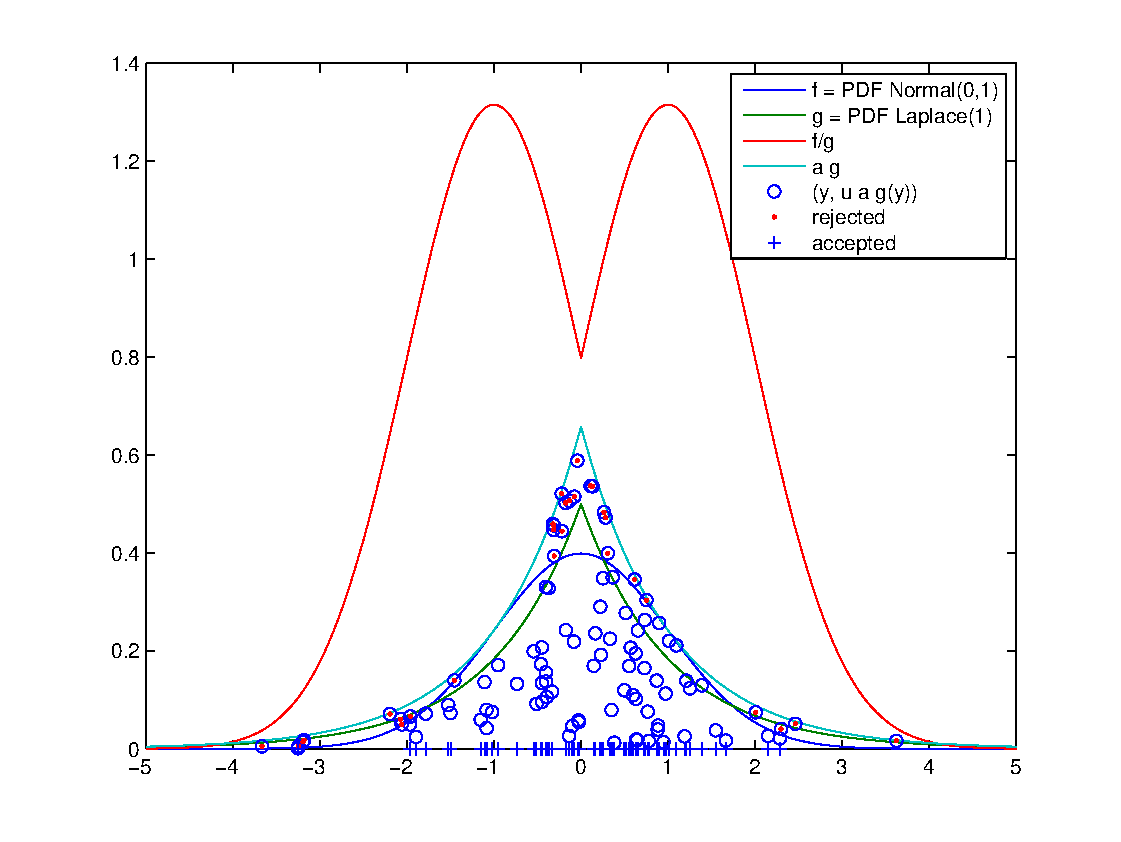
\includegraphics[width=4.50in]{figures/RSNormalLaplace}}
\end{figure}

\begin{classwork}[A note on the proposal's tail in rejection sampling]
The condition $f(x)\leq ag(x)$ is equivalent to $f(x)/g(x)\leq a$, which says that $f(x)/g(x)$ must be bounded; therefore, $g$ must have higher tails than $f$.
The rejection method cannot be used to generate from a Cauchy distribution using a normal distribution, because the latter has lower tails than the former.
\end{classwork}

%\includegraphics

The next result tells us how many iterations of the algorithm are needed, on average, to get a sample value from a RV with PDF $f$.

\begin{prop}[Acceptance Probability of RS] The expected number of iterations of the rejection algorithm to get a sample $x$ is the constant $a$.

\begin{proof}
For the continuous case:
\begin{displaymath}
\p(\textrm{`accept }y\textrm{'})=\p\left( u\leq \frac{f(y)}{ag(y)}\right)=\int^{\infty}_{-\infty}\left(\int^{f(y)/ag(y)}_0du\right)g(y)dy=\int^{\infty}_{-\infty}\frac{f(y)}{ag(y)}g(y)dy=\frac{1}{a}.
\end{displaymath}
And the number of proposals before acceptance is the $\geometric(1/a)$ RV with expectation $\frac{1}{1/a}=a$.
\end{proof}
\end{prop}

The closer $ag(x)$ is to $f(x)$, especially in the tails, the closer $a$ will be to 1, and hence the more efficient the rejection method will be.

The rejection method can still be used only if the un-normalised form of $f$ or $g$ (or both) is known. In other words, if we use:
$$f(x)=\frac{\tilde{f}(x)}{\int \tilde{f}(x)dx} \textrm{ and } g(x)=\frac{\tilde{g}(x)}{\int \tilde{g}(x)dx} $$
we know only $\tilde{f} (x)$ and/or $\tilde{g}(x)$ in closed-form.  Suppose the following are satisfied:
\begin{asparaenum}[(a)]
\item	we can generate random variables from $g$;
\item	the support of $g$ contains the support of $f$, i.e.~$\Yz \supset \Xz$;
\item	a constant $\tilde{a} > 0$ exists, such that:
\begin{equation}
\tilde{f}(x)\leq\tilde{a}\tilde{g}(x),
\end{equation}
for any $x\in \Xz$, the support of $X$.  Then $x$ can be generated from Algorithm \ref*{A:RS2}.
\end{asparaenum}

\begin{algorithm}
\caption{Rejection Sampler (RS) of von Neumann -- target shape}
\label{A:RS2}
\begin{algorithmic}[1]
\STATE {
{\it input:}
\begin{itemize}
\item[(1)] shape of a target density $\tilde{f}(x) = \left({\int \tilde{f}(x)dx}\right) f(x)$,
\item[(2)] a proposal density $g(x)$ satisfying (a), (b) and (c) above.
\end{itemize}
}
\STATE {\it output:} a sample $x$ from RV $X$ with density $f$

\REPEAT
\STATE Generate $y \sim g$ and $u \sim \uniform(0,1)$
\UNTIL{$u\leq\frac{\tilde{f}(y)}{\tilde{a}\tilde{g}(y)}$}
\STATE {\it return:} $x \gets y$
\end{algorithmic}
\end{algorithm}
Now, the expected number of iterations to get an $x$ is no longer $\tilde{a}$ but rather the integral ratio: $$ \left( \frac{\int_{\Xz} \tilde{f}(x) dx }{\int_{\Yz} \tilde{a} \tilde{g}(y) dy} \right)^{-1} \ .$$

%%The problem is already difficult for the stretched oscillating density for example.
%\begin{figure}
%\centering   \makebox[10pt]{
%\input{pqfRSMH.tex}
%}
%\caption{The characteristics of three samplers with target $p = p^*/N_p$: (1) Rejection sampler with
%proposal $q=q^*/N_q$ and the envelope function $f_q$, (2) an independent
%Metropolis-Hastings sampler (IMHS) driven by an independent base chain $I$
%with proposal $q_I = q^*_I / N_{q^*_I}$ and (3) a local Metropolis-Hastings sampler (LMHS)
%driven by a local base chain $L$ with proposal $q_L = q^*_L / N_{q^*_L}$
%centered at the current state (open square at the bottom). \label{F:RSMH}}
%\end{figure}
%Rejection Sampling from $Normal(\mu,\sigma^2)$ RV $X$ using proposals from $Cauchy(\nu)$
%\begin{model}[Cauchy]
%A RV $X$ is said to be $Cauchy(\nu)$ distributed if:
%\[
%f(x;\nu) = \frac{\nu}{\pi(x^2+\nu^2)}, \qquad F(x;\nu) = \frac{1}{2} +\frac{1}{\pi} \arctan\left(\frac{x}{\nu}\right), \qquad F^{[-1]}(u;\nu) = \nu \tan \left(\pi \left( u- \frac{1}{2} \right) \right)
%\]
%\end{model}
%\begin{labwork}
%Implement the inversion sampler to draw samples from the $Cauchy(\nu)$ RV.
%\end{labwork}

The {\bf Ziggurat Method} [G.~Marsaglia and W.~W.~Tsang, SIAM Journal of Scientific and Statistical Programming, volume 5, 1984] is a rejection sampler that can efficiently draw samples from the $Z \sim \normal(0,1)$ RV.  The \Matlab function {\tt randn} uses this method to produce samples from $Z$.\footnote{ {\tiny See \url{http://en.wikipedia.org/wiki/Ziggurat\_algorithm}} for more details.}

\begin{labwork}[Gaussian Sampling with {\tt randn}]\label{LW:randn}
We can use \Matlab function {\tt randn} that implements the Ziggurat method to draw samples from an RV $Z \sim \normal(0,1)$ as follows:
\begin{VrbM}
>> randn('state',67678); % initialise the seed at 67678 and method as Ziggurat -- TYPE help randn
>> randn % produce 1 sample from Normal(0,1) RV
ans =    1.5587
>> randn(2,8) % produce an 2 X 8 array of samples from Normal(0,1) RV
ans =
    1.2558    0.7834    0.6612    0.3247    0.1407    1.0562    0.8034    1.2970
   -0.5317    0.0417   -0.3454    0.6182   -1.4162    0.4796   -1.5015    0.3718
\end{VrbM}
If we want to produce samples from $X \sim \normal(\mu,\sigma^2)$ with some user-specified $\mu$ and $\sigma$, then we can use the following relationship between $X$ and $Z \sim \normal(0,1)$:
\[
X \gets \mu + \sigma Z, \qquad Z \sim \normal(0,1) \ .
\]
Suppose we want samples from $X \sim \normal(\mu=\pi, \sigma^2=2)$, then we can do the following:
\begin{VrbM}
>> randn('state',679); % initialise the seed at 679 and method as Ziggurat -- TYPE help randn
>> mu=pi % set the desired mean parameter mu
mu =    3.1416
>> sigma=sqrt(2) % set the desired standard deviation parameter sigma
sigma =    1.4142
>> mu + sigma * randn(2,8) % produces a 2 X 8 array of samples from Normal(3.1416,1.4.42)
ans =
    1.3955    1.7107    3.9572    3.2618    6.1652    2.6971    2.4940    4.5928
    0.8442    4.7617    3.5397    5.0282    1.6139    5.0977    2.0477    2.3286
\end{VrbM}
\end{labwork}

%%% new content added on 28 Dec 2010: Raaz to integrate and streamline
%%% this may be used as labwork or exercise, i am calling it labwork for now
\begin{labwork}[Sampling from truncated normal distributions] [Christian P. Robert, Simulation of truncated normal variables, Statistics and Computing (1995) 5, 121-125]
Let $N_+(\mu,\tau,\sigma^2)$ denote the left-truncated normal distribution with truncation point $\tau$ and density given by

$$f(x|\mu,\tau,\sigma^2)=\frac{exp(-(x-\mu)^2/2\sigma^2)}{\sqrt{2\pi}\sigma[1-\Phi((\tau-\mu)/\sigma)]}\BB{1}_{x\geq\tau}.$$

When $\tau<\mu$, the rejection sampler can readily be used to simulate from $N_+(\mu,\tau,\sigma^2)$ by simulating from $\normal(\mu,\sigma^2)$ until a number larger than $\tau$ is obtained. When $\tau>\mu$, however, this can be inefficient and increasingly so as $\tau$ gets further out into the right tail. In this case, a more efficient approach is to use the rejection sampler with the following translated exponential distribution as the proposal distribution:

$$g(y|\lambda,\tau)={\lambda}exp(-\lambda(y-\tau))\BB{1}_{y\geq\tau}.$$

\begin{enumerate}
\item Show that for simulating from $N_+(\mu=0,\tau,\sigma^2=1)$ when $\tau\geq0$, the best choice of $\lambda$ that maximizes the expected acceptance probability for the rejection sampler is given by
$$\lambda=\frac{\tau+\sqrt{\tau^2+4}}{2}$$
\item Find the maximum expected acceptance probabilities for the following truncation points, $\tau=0,0.5,1,1.5,2,2.5$ and 3. What can you conclude about efficiency as $\tau$ gets further out into the right tail?
\item Describe how samples from $N_+(\mu,\tau,\sigma^2)$ can be obtained by simulating from $N_+(\mu=0,\tau,\sigma^2=1)$ and using location-scale transformation.
\item A related distribution, denoted by $N_-(\mu,\tau,\sigma^2)$, is the right-truncated normal distribution truncated on the right at $\tau$. Describe how samples from $N_-(\mu,\tau,\sigma^2)$ can be obtained by simulating from an appropriate left-truncated normal distribution.
\item Write a \Matlab function that provides samples from a truncated normal distribution. The function should have the following inputs: number of samples required, left or right truncation, $\mu$, $\sigma^2$ and $\tau$.
\end{enumerate}
\end{labwork}

\section{Exercises in Simulation}\label{S:xsSimulation}
\begin{ExerciseList}
\Exercise Suppose the continuous RV $X$ has PDF:
\[
f_X(x) = \left(\pi(1+x^2) \right)^{-1}
\]
Devise an algorithm to transform samples from $\uniform(0,1)$ RV to those from $X$. Present your answer as pseudo-code.
\Answer
This is nothing but the inversion sampler for the standard Cauchy RV $X$.
\end{ExerciseList}


